\lhead{\bfseries LEARNING}

\section*{Literature Review}


Autonomous driving stands as one of the most promising prospects in today's automotive landscape~\cite{geiger2012ready}. Nevertheless, vehicles often navigate through intricate scenarios, where various actors with highly unpredictable behaviors coexist. To navigate such complex environments effectively, autonomous vehicles must process multiple facets of their surroundings, forecast environmental evolution, and devise suitable strategies or policies based on predefined objectives. Analogous to human decision-making processes, the predictive abilities and policy selection of autonomous vehicles should draw from their past learning experiences.

\gls{rl}, a subfield of Machine Learning, presents a broad spectrum of computational approaches for goal-directed learning through interaction~\cite{sutton2018reinforcement}. Particularly in recent years, when combined with Deep Learning, RL has found successful applications in numerous typical driving scenarios involving actors with unpredictable behaviors, such as other vehicles or pedestrians~\cite{deshpande2019deep, kim2020unexpected}. However, safety considerations impose constraints on these applications, necessitating a careful balance between the inherent benefits of experience-driven learning methods and adherence to safety protocols~\cite{d2020data, tipaldi2020applying}. Notably, it becomes increasingly prudent to initially train RL algorithms offline via simulators before transitioning to online learning in the actual operational environment.

The unexpected crossing of pedestrians represents one of the most common and critical scenarios in urban areas. According to data from the National Center for Statistics and Analysis~\cite{ncsa2017pedestrians}, approximately 6,000 pedestrians were fatally injured along roadways in the United States in 2017. Given the advancement of autonomous vehicles, the implementation of pedestrian collision avoidance systems assumes paramount importance. This work proposes an approach grounded in Deep Reinforcement Learning for autonomous vehicles navigating scenarios marked by unforeseen pedestrian crossing events. In addition to the imperative of pedestrian avoidance, the resulting agent must adhere to a predefined trajectory.

We adopt a continuous-time state/action space representation for the problem at hand, motivating the utilization of the \gls{ddpg} algorithm for agent training~\cite{lillicrap2015continuous}. Both training and testing of the \gls{ddpg}-based agent are conducted via numerical simulations (i.e., offline) to ensure compliance with aforementioned safety constraints. The proposed approach offers several advantages inherent to \gls{rl}-based methods, including the ability to handle complex systems or scenarios difficult to model, learning via simulators or real-world interaction, adaptability of learned policies to environmental changes, and minimal time required for control action selection from the learned policy~\cite{sutton2018reinforcement,bertsekas2021multiagent}.

While various \gls{rl}-based approaches have been applied to autonomous driving systems in literature, differences exist compared to our approach, such as the utilization of discrete action spaces that may not accurately represent real car control inputs, differences in problem formulation, and the adoption of online \gls{rl} approaches~\cite{everett2021collision,arvind2019autonomous}.



\gls{av} technologies represent a glimpse into the future of transportation, with many car manufacturers integrating new functionalities that constitute the foundation of \gls{adas}, ultimately paving the way for full autonomous driving capabilities~\cite{AD_mcKinsey}. However, amidst this progress, there are significant concerns regarding cybersecurity, which stands to become increasingly pivotal as Internet connectivity emerges as a critical enabling technology. The susceptibility of Control Area Network \gls{can} based communication and internet connections exposes vehicles to potential malicious attacks targeting onboard control units.

While the computer science community has extensively addressed cybersecurity in \glspl{av}, there remains a notable absence of contributions from the control systems perspective~\cite{cybersecurity_1}. In efforts to address this gap, recent research endeavors have implemented \gls{ekf} based architectures to mitigate potential sensor attacks~\cite{ekf_1_attack},~\cite{quinonez2020savior}. By employing a residual cumulative sum detector to monitor deviations between predicted and measured states, these approaches offer a means of detecting cyber-attacks. However, the reliance on a single threshold for detection raises concerns regarding false alarms, and strategies for mitigating the impact of detected attacks remain unexplored.

Expanding the purview of cybersecurity analysis from a control systems perspective, significant attention has been directed towards scenarios wherein the plant under scrutiny is modeled as a \gls{lti} system with corresponding control loops. Notably, in~\cite{attack_1}, the estimation and control of linear systems under cyber-attacks are examined, with the authors proposing an algorithm based on compressed sensing for reconstructing corrupted states. However, limitations emerge, as demonstrated by the impossibility of reconstructing the state of an \gls{lti} system if more than half of the sensors are compromised.

\gls{mpc} based solutions have also been explored to bolster the resilience of control loops in the face of cyber threats, as evidenced in~\cite{attack_3}  and~\cite{attack_4} . These studies implement \gls{lti}-based solutions have also been explored to bolster the resilience of control loops in the face of cyber threats, as evidenced in~\cite{attack_3}  and~\cite{attack_4} .  controllers to enhance control loop robustness when the threatened plant is assumed to be linear and time-invariant. However, while assuming \gls{lti} dynamics may not always align with the complexities of  \glspl{av}, it offers mathematical tractability, which proves advantageous for investigating the problem at hand.

\chapter{Reinforcement Learning for Collision Avoidance}
\label{Chapter:3}

As we delve into the complexities of autonomous vehicular navigation in urban settings, the challenge of ensuring pedestrian safety emerges as a critical concern. This chapter presents a comprehensive study on enhancing pedestrian collision avoidance through the application of Deep Reinforcement Learning (DRL), with a specific focus on the Deep Deterministic Policy Gradient (DDPG) algorithm. The integration of DRL in autonomous driving systems represents a paradigm shift towards more adaptive, intelligent, and safer navigation strategies that can dynamically respond to the unpredictability of urban environments. This chapter not only explores the theoretical underpinnings of DRL and its suitability for continuous state and action spaces but also provides a meticulous examination of the DDPG algorithm's architecture, highlighting its potential to revolutionize pedestrian safety mechanisms in autonomous vehicles.

The urgency for such advancements cannot be overstated, as pedestrian safety remains a paramount concern in the development of autonomous driving technologies. Traditional approaches often fall short in dynamically complex scenarios, where the ability to predict and react to pedestrian movements in real-time is crucial. The DDPG algorithm, with its capability to learn optimal policies over continuous action spaces, offers a promising solution to this problem, enabling autonomous vehicles to make nuanced decisions that significantly reduce the risk of collisions.


\newpage



This work proposes an approach based on Deep Reinforcement Learning for autonomous vehicles operating in a scenario featured by  unexpected pedestrian crossing events. Besides the capability of avoiding pedestrians, the resulting agent has to follow a given trajectory.  We adopt a continuous time state/action space representation for the problem at hand, and this choice motivates the usage of the Deep Deterministic Policy Gradient (DDPG) algorithm to train the agent~\cite{DDPG}.
%\cite{DDPG, DDPG_vehicle}. 
Both the training and the testing of the DDPG based agent are performed via numerical simulations (i.e., off-line) in order to meet the above mentioned safety constraints. The main advantages of using the proposed approach also resides in the typical benefits of applying RL based methods, such as the possibility of dealing with complex systems/scenarios difficult to be modelled, the possibility of learning via simulators or by interacting with the real environment, the adaptability of the learnt policy to the environment changes (thanks to RL intrinsic on-line continuous learning capabilities), the negligible time needed to select the control action from the learnt policy~\cite{sutton2018reinforcement, bertsekas2021multiagent}. In literature, we can find different RL based approaches applied to autonomous driving systems. However, some differences versus our approach can be noticed, such as the usage of discrete action spaces which does not represent accurately the real car control inputs, the problem formulation, and the adoption of on-line RL approaches~\cite{everett2021collision, arvind2019autonomous}. 






%where $s'$ indicates all the possible next states from $s$ according to $P(\cdot|s,a)$.

%\color{blue}
%Ora dobbiamo passare alla versione campionata...dove l'operatore expectation dovrebbe essere tolto. In realtà stiamo facendo una media su campioni. Dire in qualche modo che stiamo facendo la media campionata.
%\color{black}





\section{The proposed RL system for the  pedestrian collision avoidance problem}
\label{sec:Envinronment formalization}
%\color{blue}
%Chiarire cosa diventa P e R nel nostro caso: R è deterministica, la policy anche, la P non è nota, e andrebbe ricercata nel pedone. Il modello del veicolo serve dato che stiamo facendo un training in un ambiente simulation.
%\color{green}
%@Massimo Anche questo dovrebbe essere fatto
%\color{black}
This section describes all the elements of the RL system for the pedestrian collision avoidance problem, including the reward function definition. Both the agent architecture and the environment model are described, the latter needed for training and testing the DDPG based agent via numerical simulations.

We consider the intersection scenario shown in \mbox{Fig.~\ref{fig:scenario}},  where an autonomous vehicle has to follow a straight trajectory planned by a local path planner and to manage unexpected pedestrian crossings. A DDPG based agent is designed and trained to achieve such two competing objectives.  

%unexpectedly a pedestrian crosses the road during its red light. This scenario was inspired by the statistics of the NHTSA report \cite{NTHSA}, which sheds light on the danger of such situations. The goal of this paper is to show how an RL agent can learn to avoid the two task simultaneously: pedestrian avoidance and track a planned trajectory.

\begin{figure}[ht] 
	\centering
\tikzset{every picture/.style={line width=0.75pt}} %set default line width to 0.75pt        

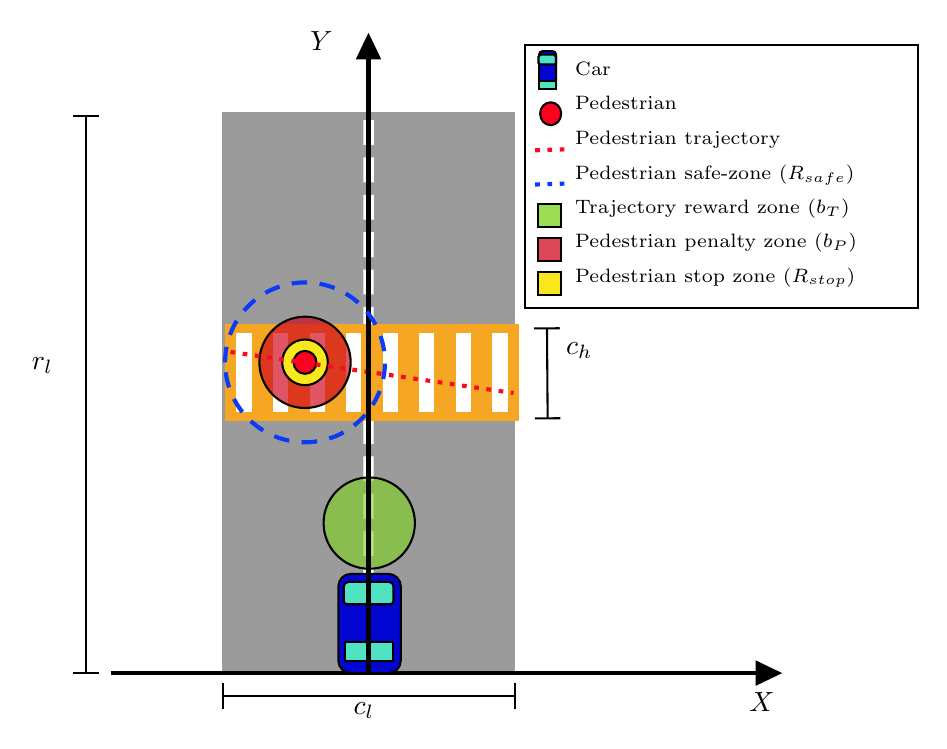
\begin{tikzpicture}[x=0.75pt,y=0.75pt,yscale=-1.1,xscale=1.1]
	%uncomment if require: \path (0,390); %set diagram left start at 0, and has height of 390
	
	%Straight Lines [id:da28584899643381045] 
	\draw [color={rgb, 255:red, 0; green, 0; blue, 0 }  ,draw opacity=1 ][fill={rgb, 255:red, 208; green, 2; blue, 27 }  ,fill opacity=1 ][line width=1.5]    (62,281) -- (352,281) ;
	\draw [shift={(356,281)}, rotate = 180] [fill={rgb, 255:red, 0; green, 0; blue, 0 }  ,fill opacity=1 ][line width=0.08]  [draw opacity=0] (11.61,-5.58) -- (0,0) -- (11.61,5.58) -- cycle    ;
	%Shape: Rectangle [id:dp5180666136146594] 
	\draw  [draw opacity=0][fill={rgb, 255:red, 155; green, 155; blue, 155 }  ,fill opacity=1 ] (238.84,280) -- (238.84,35.24) -- (110.84,35.24) -- (110.84,280) -- cycle ;
	%Straight Lines [id:da5379043576147695] 
	\draw [color={rgb, 255:red, 255; green, 255; blue, 255 }  ,draw opacity=1 ][fill={rgb, 255:red, 255; green, 255; blue, 255 }  ,fill opacity=1 ][line width=3.75]  [dash pattern={on 9pt off 4.5pt}]  (174.86,38.77) -- (174.82,277.88) ;
	%Shape: Rectangle [id:dp5984726439545023] 
	\draw  [draw opacity=0][fill={rgb, 255:red, 245; green, 166; blue, 35 }  ,fill opacity=1 ] (112.04,128.11) -- (240.71,128.11) -- (240.71,170.55) -- (112.04,170.55) -- cycle ;
	%Shape: Rectangle [id:dp3598384588943413] 
	\draw  [draw opacity=0][fill={rgb, 255:red, 255; green, 255; blue, 255 }  ,fill opacity=1 ] (117,132) -- (123.71,132) -- (123.71,166.45) -- (117,166.45) -- cycle ;
	%Shape: Rectangle [id:dp42660139670374453] 
	\draw  [draw opacity=0][fill={rgb, 255:red, 255; green, 255; blue, 255 }  ,fill opacity=1 ] (133,132) -- (139.71,132) -- (139.71,166.45) -- (133,166.45) -- cycle ;
	%Shape: Rectangle [id:dp4481761265320998] 
	\draw  [draw opacity=0][fill={rgb, 255:red, 255; green, 255; blue, 255 }  ,fill opacity=1 ] (149,132) -- (155.71,132) -- (155.71,166.45) -- (149,166.45) -- cycle ;
	%Shape: Rectangle [id:dp31095403090704243] 
	\draw  [draw opacity=0][fill={rgb, 255:red, 255; green, 255; blue, 255 }  ,fill opacity=1 ] (165,132) -- (171.71,132) -- (171.71,166.45) -- (165,166.45) -- cycle ;
	%Shape: Rectangle [id:dp9559285707259317] 
	\draw  [draw opacity=0][fill={rgb, 255:red, 255; green, 255; blue, 255 }  ,fill opacity=1 ] (181,132) -- (187.71,132) -- (187.71,166.45) -- (181,166.45) -- cycle ;
	%Shape: Rectangle [id:dp21507599882927209] 
	\draw  [draw opacity=0][fill={rgb, 255:red, 255; green, 255; blue, 255 }  ,fill opacity=1 ] (197,132) -- (203.71,132) -- (203.71,166.45) -- (197,166.45) -- cycle ;
	%Shape: Rectangle [id:dp041486191842157405] 
	\draw  [draw opacity=0][fill={rgb, 255:red, 255; green, 255; blue, 255 }  ,fill opacity=1 ] (213,132) -- (219.71,132) -- (219.71,166.45) -- (213,166.45) -- cycle ;
	%Shape: Rectangle [id:dp7164243700354131] 
	\draw  [draw opacity=0][fill={rgb, 255:red, 255; green, 255; blue, 255 }  ,fill opacity=1 ] (229,132) -- (235.71,132) -- (235.71,166.45) -- (229,166.45) -- cycle ;
	%Flowchart: Connector [id:dp4051301354453565] 
	\draw  [fill={rgb, 255:red, 208; green, 2; blue, 27 }  ,fill opacity=0.67 ] (127.02,144.89) .. controls (127.02,133.85) and (135.97,124.89) .. (147.02,124.89) .. controls (158.07,124.89) and (167.02,133.85) .. (167.02,144.89) .. controls (167.02,155.94) and (158.07,164.89) .. (147.02,164.89) .. controls (135.97,164.89) and (127.02,155.94) .. (127.02,144.89) -- cycle ;
	%Flowchart: Connector [id:dp9639108171950941] 
	\draw  [fill={rgb, 255:red, 248; green, 231; blue, 28 }  ,fill opacity=1 ] (137.02,144.89) .. controls (137.02,139.37) and (141.5,134.89) .. (147.02,134.89) .. controls (152.54,134.89) and (157.02,139.37) .. (157.02,144.89) .. controls (157.02,150.41) and (152.54,154.89) .. (147.02,154.89) .. controls (141.5,154.89) and (137.02,150.41) .. (137.02,144.89) -- cycle ;
	%Flowchart: Connector [id:dp4727997208074779] 
	\draw  [fill={rgb, 255:red, 255; green, 0; blue, 31 }  ,fill opacity=1 ] (142.02,144.89) .. controls (142.02,142.13) and (144.26,139.89) .. (147.02,139.89) .. controls (149.78,139.89) and (152.02,142.13) .. (152.02,144.89) .. controls (152.02,147.65) and (149.78,149.89) .. (147.02,149.89) .. controls (144.26,149.89) and (142.02,147.65) .. (142.02,144.89) -- cycle ;
	%Straight Lines [id:da041073960472972626] 
	\draw [color={rgb, 255:red, 248; green, 10; blue, 39 }  ,draw opacity=1 ][line width=1.5]  [dash pattern={on 1.69pt off 2.76pt}]  (114.37,140.33) -- (238.37,158.33) ;
	%Shape: Rectangle [id:dp15185882367612136] 
	\draw   (243.29,6) -- (415.5,6) -- (415.5,121.2) -- (243.29,121.2) -- cycle ;
	%Straight Lines [id:da7988843189062504] 
	\draw [color={rgb, 255:red, 248; green, 10; blue, 39 }  ,draw opacity=1 ][line width=1.5]  [dash pattern={on 1.69pt off 2.76pt}]  (247.82,52) -- (262.25,51.55) ;
	%Flowchart: Connector [id:dp7590194899937404] 
	\draw  [fill={rgb, 255:red, 255; green, 0; blue, 31 }  ,fill opacity=1 ] (250,36) .. controls (250,33.24) and (252.06,31) .. (254.61,31) .. controls (257.15,31) and (259.21,33.24) .. (259.21,36) .. controls (259.21,38.76) and (257.15,41) .. (254.61,41) .. controls (252.06,41) and (250,38.76) .. (250,36) -- cycle ;
	%Shape: Rectangle [id:dp20536350583269547] 
	\draw  [fill={rgb, 255:red, 126; green, 211; blue, 33 }  ,fill opacity=0.77 ] (249,75.5) -- (259,75.5) -- (259,85.5) -- (249,85.5) -- cycle ;
	%Shape: Rectangle [id:dp7543763695429884] 
	\draw  [fill={rgb, 255:red, 248; green, 231; blue, 28 }  ,fill opacity=1 ] (249,105.5) -- (259,105.5) -- (259,115.5) -- (249,115.5) -- cycle ;
	%Straight Lines [id:da9289731261582568] 
	\draw    (51,37) -- (51,281) ;
	\draw [shift={(51,281)}, rotate = 270] [color={rgb, 255:red, 0; green, 0; blue, 0 }  ][line width=0.75]    (0,5.59) -- (0,-5.59)   ;
	\draw [shift={(51,37)}, rotate = 270] [color={rgb, 255:red, 0; green, 0; blue, 0 }  ][line width=0.75]    (0,5.59) -- (0,-5.59)   ;
	%Straight Lines [id:da5378932582334461] 
	\draw    (239,291) -- (111,291) ;
	\draw [shift={(111,291)}, rotate = 360] [color={rgb, 255:red, 0; green, 0; blue, 0 }  ][line width=0.75]    (0,5.59) -- (0,-5.59)   ;
	\draw [shift={(239,291)}, rotate = 360] [color={rgb, 255:red, 0; green, 0; blue, 0 }  ][line width=0.75]    (0,5.59) -- (0,-5.59)   ;
	%Straight Lines [id:da33109690518949986] 
	\draw    (253,130) -- (253.29,169.41) ;
	\draw [shift={(253.29,169.41)}, rotate = 269.58] [color={rgb, 255:red, 0; green, 0; blue, 0 }  ][line width=0.75]    (0,5.59) -- (0,-5.59)   ;
	\draw [shift={(253,130)}, rotate = 269.58] [color={rgb, 255:red, 0; green, 0; blue, 0 }  ][line width=0.75]    (0,5.59) -- (0,-5.59)   ;
	%Flowchart: Connector [id:dp6794245955836984] 
	\draw  [fill={rgb, 255:red, 126; green, 211; blue, 33 }  ,fill opacity=0.61 ] (155.15,215.3) .. controls (155.15,204.25) and (164.1,195.3) .. (175.15,195.3) .. controls (186.2,195.3) and (195.15,204.25) .. (195.15,215.3) .. controls (195.15,226.34) and (186.2,235.3) .. (175.15,235.3) .. controls (164.1,235.3) and (155.15,226.34) .. (155.15,215.3) -- cycle ;
	%Rounded Rect [id:dp7752804182072381] 
	\draw  [fill={rgb, 255:red, 2; green, 6; blue, 208 }  ,fill opacity=1 ] (183.5,237.55) .. controls (186.52,237.55) and (188.97,240) .. (188.97,243.02) -- (188.97,275.53) .. controls (188.97,278.55) and (186.52,281) .. (183.5,281) -- (167.1,281) .. controls (164.08,281) and (161.63,278.55) .. (161.63,275.53) -- (161.63,243.02) .. controls (161.63,240) and (164.08,237.55) .. (167.1,237.55) -- cycle ;
	%Rounded Same Side Corner Rect [id:dp6191447553378682] 
	\draw  [fill={rgb, 255:red, 80; green, 227; blue, 194 }  ,fill opacity=1 ] (164,243.02) .. controls (164,241.94) and (164.88,241.06) .. (165.96,241.06) -- (183.82,241.06) .. controls (184.9,241.06) and (185.78,241.94) .. (185.78,243.02) -- (185.78,249.37) .. controls (185.78,250.18) and (185.12,250.85) .. (184.3,250.85) -- (165.48,250.85) .. controls (164.66,250.85) and (164,250.18) .. (164,249.37) -- cycle ;
	%Shape: Rectangle [id:dp15584204124077772] 
	\draw  [fill={rgb, 255:red, 80; green, 227; blue, 194 }  ,fill opacity=1 ] (164.5,267.55) -- (185.61,267.55) -- (185.61,275.53) -- (164.5,275.53) -- cycle ;
	%Shape: Rectangle [id:dp7507189763383675] 
	\draw  [fill={rgb, 255:red, 208; green, 2; blue, 27 }  ,fill opacity=0.73 ] (249,90.5) -- (259,90.5) -- (259,100.5) -- (249,100.5) -- cycle ;
	%Straight Lines [id:da3637152716158101] 
	\draw [color={rgb, 255:red, 0; green, 0; blue, 0 }  ,draw opacity=1 ][fill={rgb, 255:red, 208; green, 2; blue, 27 }  ,fill opacity=1 ][line width=1.5]    (174.82,281) -- (174.82,4.55) ;
	\draw [shift={(174.82,0.55)}, rotate = 450] [fill={rgb, 255:red, 0; green, 0; blue, 0 }  ,fill opacity=1 ][line width=0.08]  [draw opacity=0] (11.61,-5.58) -- (0,0) -- (11.61,5.58) -- cycle    ;
	%Shape: Circle [id:dp43448679482079333] 
	\draw  [color={rgb, 255:red, 11; green, 58; blue, 249 }  ,draw opacity=1 ][dash pattern={on 5.63pt off 4.5pt}][line width=1.5]  (112.02,144.89) .. controls (112.02,125.56) and (127.69,109.89) .. (147.02,109.89) .. controls (166.35,109.89) and (182.02,125.56) .. (182.02,144.89) .. controls (182.02,164.22) and (166.35,179.89) .. (147.02,179.89) .. controls (127.69,179.89) and (112.02,164.22) .. (112.02,144.89) -- cycle ;
	%Rounded Rect [id:dp8343624362355313] 
	\draw  [fill={rgb, 255:red, 2; green, 6; blue, 208 }  ,fill opacity=1 ] (255.47,8.59) .. controls (256.29,8.59) and (256.96,9.26) .. (256.96,10.08) -- (256.96,23.59) .. controls (256.96,24.41) and (256.29,25.08) .. (255.47,25.08) -- (251.01,25.08) .. controls (250.19,25.08) and (249.52,24.41) .. (249.52,23.59) -- (249.52,10.08) .. controls (249.52,9.26) and (250.19,8.59) .. (251.01,8.59) -- cycle ;
	%Shape: Rectangle [id:dp893778457744719] 
	\draw  [fill={rgb, 255:red, 80; green, 227; blue, 194 }  ,fill opacity=1 ] (249.52,21.61) -- (256.96,21.61) -- (256.96,25.08) -- (249.52,25.08) -- cycle ;
	%Rounded Same Side Corner Rect [id:dp9092713415456457] 
	\draw  [fill={rgb, 255:red, 80; green, 227; blue, 194 }  ,fill opacity=1 ] (249.29,10.97) .. controls (249.29,10.5) and (249.67,10.12) .. (250.14,10.12) -- (256.11,10.12) .. controls (256.58,10.12) and (256.96,10.5) .. (256.96,10.97) -- (256.96,13.72) .. controls (256.96,14.08) and (256.67,14.36) .. (256.32,14.36) -- (249.93,14.36) .. controls (249.58,14.36) and (249.29,14.08) .. (249.29,13.72) -- cycle ;
	%Straight Lines [id:da6017239908080465] 
	\draw [color={rgb, 255:red, 11; green, 58; blue, 249 }  ,draw opacity=1 ][line width=1.5]  [dash pattern={on 1.69pt off 2.76pt}]  (247.82,67) -- (262.25,66.55) ;
	
	% Text Node
	\draw (340.33,288.23) node [anchor=north west][inner sep=0.75pt]  [color={rgb, 255:red, 0; green, 0; blue, 0 }  ,opacity=1 ]  {$X$};
	% Text Node
	\draw (148,-1.24) node [anchor=north west][inner sep=0.75pt]  [color={rgb, 255:red, 0; green, 0; blue, 0 }  ,opacity=1 ]  {$Y$};
	% Text Node
	\draw (264,42) node [anchor=north west][inner sep=0.75pt]  [font=\scriptsize] [align=left] {Pedestrian trajectory};
	% Text Node
	\draw (264,27) node [anchor=north west][inner sep=0.75pt]  [font=\scriptsize] [align=left] {Pedestrian};
	% Text Node
	\draw (264,72) node [anchor=north west][inner sep=0.75pt]  [font=\scriptsize] [align=left] {Trajectory reward zone $(b_T)$ };
	% Text Node
	\draw (264,102) node [anchor=north west][inner sep=0.75pt]  [font=\scriptsize] [align=left] {Pedestrian stop zone $(R_{stop})$};
	% Text Node
	\draw (26,141.41) node [anchor=north west][inner sep=0.75pt]    {$r_{l}$};
	% Text Node
	\draw (167,292.41) node [anchor=north west][inner sep=0.75pt]    {$c_{l}$};
	% Text Node
	\draw (260,134.95) node [anchor=north west][inner sep=0.75pt]    {$c_{h}$};
	% Text Node
	\draw (264,87) node [anchor=north west][inner sep=0.75pt]  [font=\scriptsize] [align=left] {Pedestrian penalty zone $(b_P)$};
	% Text Node
	\draw (264,12) node [anchor=north west][inner sep=0.75pt]  [font=\scriptsize] [align=left] {Car};
	% Text Node
	\draw (264,57) node [anchor=north west][inner sep=0.75pt]  [font=\scriptsize] [align=left] {Pedestrian safe-zone ($R_{safe}$)};
	
	
\end{tikzpicture}
\caption{The intersection scenario for the pedestrian collision avoidance problem.}
\label{fig:scenario}
\end{figure}

More specifically, such scenario is composed by a straight road (with length $r_l= \SI{50}{\metre}$ and width $c_l=\SI{10}{\metre}$) and a crosswalk area (perpendicular to the road direction and placed at $\frac{r_l}{2}$ with a height of $c_h= \SI{2.5}{\metre}$). The vehicle has to follow the reference trajectory depicted as dashed white line in Fig.~\ref{fig:scenario}. During any travelling episode along the road, a pedestrian can unexpectedly cross the road when the traffic light allows the vehicle to proceed. 

\begin{figure}[ht]
\centering
\tikzset{every picture/.style={line width=0.75pt}} %set default line width to 0.75pt    
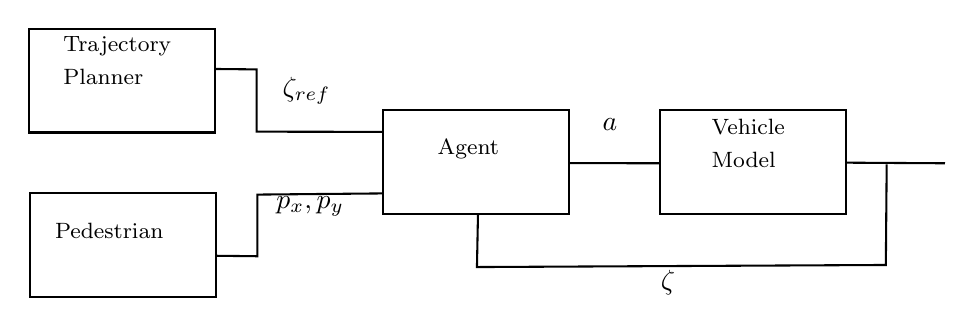
\begin{tikzpicture}[x=0.75pt,y=0.75pt,yscale=-1,xscale=1]
	%Shape: Rectangle [id:dp11457776888363957] 
	\draw   (77.13,55.6) -- (166.92,55.6) -- (166.92,105.6) -- (77.13,105.6) -- cycle ;
	%Shape: Rectangle [id:dp14347854375529412] 
	\draw   (247.67,94.93) -- (337.45,94.93) -- (337.45,144.93) -- (247.67,144.93) -- cycle ;
	%Shape: Rectangle [id:dp7094628553182183] 
	\draw   (381.17,94.9) -- (470.95,94.9) -- (470.95,144.9) -- (381.17,144.9) -- cycle ;
	%Shape: Rectangle [id:dp4842733937121826] 
	\draw   (77.67,134.93) -- (167.45,134.93) -- (167.45,184.93) -- (77.67,184.93) -- cycle ;
	%Straight Lines [id:da08669167245414444] 
	\draw    (167,75) -- (186.93,75.2) -- (186.93,105.2) -- (248.04,105.3) ;
	%Straight Lines [id:da9567989410678546] 
	\draw    (167.86,165) -- (187.3,165.22) -- (187.27,135.52) -- (247.84,134.95) ;
	%Straight Lines [id:da542342739302786] 
	\draw    (337.41,120.35) -- (381.09,120.43) ;
	%Straight Lines [id:da8872076809294023] 
	\draw    (471.05,120.14) -- (518.59,120.43) ;
	%Straight Lines [id:da75203079626961] 
	\draw    (490.5,121) -- (490.09,169.43) -- (293.09,170.43) -- (293.59,144.93) ;
	
	% Text Node
	\draw (92.3,57.67) node [anchor=north west][inner sep=0.75pt]   [align=left] {{\footnotesize Trajectory}\\{\footnotesize Planner}};
	% Text Node
	\draw (88.33,147.67) node [anchor=north west][inner sep=0.75pt]   [align=left] {{\footnotesize Pedestrian}};
	% Text Node
	\draw (272.7,107.5) node [anchor=north west][inner sep=0.75pt]   [align=left] {{\footnotesize Agent}};
	% Text Node
	\draw (404.67,97.5) node [anchor=north west][inner sep=0.75pt]   [align=left] {{\footnotesize Vehicle}\\{\footnotesize Model}};
	% Text Node
	\draw (198,77.33) node [anchor=north west][inner sep=0.75pt]    {${\textstyle \zeta _{ref}}$};
	% Text Node
	\draw (352.17,97.5) node [anchor=north west][inner sep=0.75pt]    {$a$};
	% Text Node
	\draw (380.17,170.5) node [anchor=north west][inner sep=0.75pt]    {$\zeta $};
	% Text Node
	\draw (195,135) node [anchor=north west][inner sep=0.75pt]    {$p_{x} ,p_{y}$};
\end{tikzpicture}
\caption{The agent-environment interaction for the pedestrian collision avoidance problem.}
\label{fig:principle_scheme}
\end{figure}
In such a situation, the trained DDPG based agent has to command the vehicle to avoid the inattentive pedestrian, and then taking again the reference trajectory. The overall RL system has been implemented in Matlab/Simulink. It consists of the DDPG based agent and its environment, that is to say, the vehicle itself, the pedestrian, and the trajectory planner (see Fig.~\ref{fig:principle_scheme}). The agent interacts with its environment through the vehicle acceleration and steering commands. The stochastic nature of the proposed system is linked to the unexpected behaviour of the pedestrian, who can enter the crosswalk area at any time and by following an unknown path within such area. In other words, while learning to follow the reference trajectory, the effect of the selected sequence of actions on the expected return $G_t$ is subject to such unknown pedestrian behaviour.
%are not deterministically  we do not have the $P(\cdot|s,a)$ especially around the pedestrian crossing and this makes it necessary to use learning techniques to approximate the \textit{Q-function} such as \textit{DDPG}. The reward $R(\cdot|s,a)$, on the other hand, is deterministic and is carefully designed to guide the \texit{Q-learning} process so that the agent is able to perform his task.
%In the remaining part of this section, all the elements of the proposed RL system are described, including the reward function definition.
%the various components of the RL system are described in detail. In particular the model of the car and the trajectory planner are reported in section \ref{sub_sec:3-a} and \ref{sub_sec:3-b} respectively, the behaviour of the pedestrian is described in section \ref{sub_sec:3-c}, the details on the implementation of the agent are reported in section \ref{sub_sec:3-d} and the reward shaping is characterized in section \ref{sub_sec:3-e}.
\begin{figure}[ht]
\centering
\includegraphics[scale=0.5]{figure/Part2/Chapter5/Images/model_vehicle.jpg} 
\caption{The vehicle model.}
\label{fig:model_vehicle}
\end{figure}

\subsection{The vehicle dynamics model}
\label{sub_sec:3-a}
Vehicles operating in an urban environment can be represented via a kinematic based model~\cite{bicycle_Frazzoli}. In this work, we adopt the model described in~\cite{bicycle_Borrelli}, which is shown in \mbox{Fig.~\ref{fig:model_vehicle}}. In such model, the wheels do not slip at their contact point with the ground since both the velocity and the acceleration values are assumed to be low. 
The following set of nonlinear continuous time equations describes the selected model for the vehicles dynamics
\begin{subequations}
\label{vehicmodel}
\begin{align}
	\frac{dx(t)}{dt} &=v(t) \cos (\psi(t)+\beta(t)), \\
	\frac{dy(t)}{dt} &=v(t) \sin (\psi(t)+\beta(t)), \\
	\frac{d\psi(t)}{dt} &=\frac{v(t)}{l_{r}} \sin (\beta(t)), \\
	\frac{dv(t)}{dt} &= \mu(t), 
\end{align}
\end{subequations}
\noindent with
\begin{subequations}[resume]
\begin{align}
	\beta(t) &=\tan ^{-1}\left(\frac{l_{r}}{l_{f}+l_{r}} \tan \left(\delta_{f}(t)\right)\right).
\end{align}
\end{subequations}
In our work, for the sake of simplicity, we make explicit the time  dependence of the state and action variables only when they are introduced for the first time. In the presented model, $x$ and $y$ are the vehicle mass-center coordinates in an inertial frame, while the heading angle and the speed of the vehicle mass-center are $\psi$ and $v$. The distance from the vehicle mass-center to the front and rear axles are $l_f= \SI{1.738}{\metre}$ and $l_r=\SI{1.105}{\metre}$, respectively. Moreover, $\beta$ represents the angle of the current mass-center velocity vector with respect to the longitudinal axis of
the vehicle, while $\mu$ is the mass-center acceleration along such velocity vector. The control inputs are the front steering angles $\delta_f$ and the acceleration $\mu$. In other words, we assume that the vehicle is a front wheel steering vehicle, hence $\delta_r \equiv 0$.   

The vehicle dynamics model~\eqref{vehicmodel}  can be expressed in a vector form as follows
\begin{equation}
\begin{aligned}
	\frac{d\zeta}{dt}  & = f(\zeta,u), \\
	%\zeta  \in & \mathbf{R}^{n_\zeta} , u \in \mathbf{R}^{n_u}. \\
\end{aligned}
\end{equation}
\noindent where $\zeta=[x,y, \psi, v]' \in {R}^{4}$ and $u=[\delta_f ,\mu]' \in {R}^{2}$ represent the state and input vector, respectively (note that the \mbox{symbol $'$} denotes the transpose operator).


\subsection{The pedestrian position and the trajectory planner}
\label{sub_sec:3-b}
The pedestrian position measurements are described by the following equations
\begin{equation}
\begin{cases} p_x(t)=p_{x_0}+v_{x_p}\cdot t+\eta_{ \rm x}, \\ p_y(t)=p_{y_0}+v_{y_p}\cdot t +\eta_{\rm y},
\end{cases} 
\end{equation}
where
\begin{itemize}
\item $p_{x_0}$ and $p_{y_0}$ are the  coordinates of the pedestrian initial position. 
\item $v_{x_p}$ and $v_{y_p}$ are the component of the pedestrian velocity vector and are assumed to be constant.
\item $\eta_{\rm x} \sim \mathcal{N}\left(0, \sigma_{\rm \eta_x}^{2}\right)$ and $ \eta_{\rm y} \sim \mathcal{N}\left(0, \sigma_{\rm \eta_y}^{2}\right)$ represent the Gaussian noise of the vehicle on-board devices (e.g., RADAR sensors), responsible for the acquisition of the current pedestrian position $p = [p_x, p_y]'$. 
%By considering that the pedestrian position can be acquired by vehicle on-board devices (e.g., RADAR sensors), we add their related measurement Gaussian noise $\eta_{radar} \sim \mathcal{N}\left(0, \sigma_{radar}^{2}\right)$ when computing the current pedestrian position $p(t) = [p_x(t), p_y(t)]'$.
\end{itemize}

We set the values of the pedestrian initial and final position vectors, $p_0=[p_{x_0}, p_{y_0}]'$ and $p_f=[p_{x_f}, p_{y_f}]'$, as follows
\begin{itemize}
\item $p_{x_f} $ and $p_{x_0}$ are chosen according to a Bernoulli random variable $b \sim \operatorname{Bern}(0.5)$ as
\begin{equation}
	\centering   
	\begin{aligned}
		p_{x_f} & =-(2b-1)\cdot\frac{c_l}{2}, \\
		p_{x_0} & =(2b-1)\cdot\frac{c_l}{2};
	\end{aligned}
\end{equation}
\item $p_{y_f} $ and $p_{y_0}$ are Gaussian random variables, namely $p_{y_f} \sim \mathcal{N}\left(\frac{r_l}{2}, \sigma_{y}^2\right)$, $p_{y_0} \sim \mathcal{N}\left(\frac{r_l}{2},\sigma_{y}^2\right)$.
\end{itemize}

The variances $\sigma_{\rm \eta_x}^2 = \sigma_{\rm \eta_y}^2$ and $\sigma_{y}^2$ are set to $\SI{0.2}{m^2}$ and $\SI{1}{m^2}$, respectively. The pedestrian moves along a straight path within the crosswalk area at the constant velocity vector $v_p=[v_{x_p}, v_{y_p}]'$.
%, which can be easily computed once we set the departure and arrival times ($t_0$ and $t_f$) for the given episode. They are chosen in such a way that the vehicle can potentially hit the pedestrian along its trajectory. 




%\begin{equation}
%    v_p=\frac{p_f-p_0 }{t_f-t_0}
%\end{equation}
%where $p_f=[p_{x_f} \quad p_{y_f}]'$ and $p_0=[p_{x_0} \quad p_{y_0}]'$. Where   $p_{x_f} $ and $p_{x_0}$ are chosen according to a Bernoulli random variable $b \sim \operatorname{Bern}(0.5)$ as:
%\begin{equation}
% \centering   
%\begin{aligned}
%    p_{x_f} & =-(2b-1)\cdot\frac{c_l}{2} \\
%    p_{x_0} & =(2b-1)\cdot\frac{c_l}{2}
%\end{aligned}
%\end{equation}
%and $p_{y_f} $ and $p_{y_0}$ are gaussian random variables namely $p_{y_f} \sim \mathcal{N}\left(\frac{r_l}{2}, \sigma_{y}\right)$, $p_{y_0} \sim \mathcal{N}\left(\frac{r_l}{2},\sigma_{y}\right)$.




%\subsection{Trajectory planner}
\label{sub_sec:3-c}
The local trajectory planner calculates a uniform rectilinear motion  $\zeta_{\rm ref}(t)=[x_{ref}(t) ,y_{\rm ref}(t),\psi_{\rm ref}(t),v_{\rm ref}(t)]' $ that the vehicle has to follow
\begin{equation}
\centering
\begin{aligned}
	x_{\rm ref}(t)&=0, \\ 
	y_{\rm ref}(t) &=  v_{\rm const} \cdot \sin{\psi_{\rm const}} \cdot t, \\
	v_{\rm ref}(t) &= v_{\rm const}, \\
	\psi_{\rm ref}(t) &= \psi_{\rm const}.
\end{aligned}
\end{equation}



In our training episodes, we set the reference cruise velocity $v_{\rm const}$ to $\SI{10}{\frac{\metre}{\sec}}$ and the reference heading direction $\psi_{\rm ref}$ to $\frac{\pi}{2}$ \SI{}{\radian} . 



\subsection{The proposed DDPG based agent architecture}
\label{sub_sec:3-d}
The proposed DDPG based agent processes the following two error vectors
\begin{equation}
\centering   
\begin{aligned}
	e_T(t) &= [ x_{\rm ref}(t)-x(t), y_{\rm ref}(t)-y(t)]',  \\
	e_P(t) &= [p_x(t)-x(t), p_y(t)-y(t)]',  \\
\end{aligned}
\end{equation}
\noindent where $e_T$ and $e_P$ are  the error of the autonomous vehicle with respect to the reference trajectory and its relative distance to the pedestrian, respectively. Hence, the continuous time state and action vectors for the DDPG based agent can be expressed as follows  
\begin{equation}
\label{Eq:state_action}
\begin{aligned}
	s(t)=&[e_T(t), \frac{de_T(t)}{dt}, e_P(t), \frac{de_P(t)}{dt}]', \\
	a(t)=&[\delta_f(t), \mu(t)]'.
\end{aligned}
\end{equation}

In this work, we use the agent architecture shown in Fig.~\ref{fig:act_crit}. The neural networks are composed of fully connected layers with $N_{\rm nn}=100$ number of neurons.
%in Fig. \ref{Critic_Network} and Fig. \ref{Actor_Network}, where {\rm FC} and {\rm TL} represent the fully connected layers and activation function $\tanh$ layers.
%Each fully connected layer consists of $N_{nn}=100$ number of neurons.
%\begin{figure}[ht]
%	\centering
%	\includegraphics[scale=0.23]{Images/nn.jpg} 
%	\caption{Critic network of the proposed DDPG based agent.}
%	\label{Critic_Network}
%\end{figure}
%\begin{figure}[ht]
%	\centering
%	\includegraphics[scale=0.23]{Images/act.png} 
%	\caption{Actor network of the proposed DDPG based agent.}
%	\label{Actor_Network}
%\end{figure}
The DDPG algorithm~\cite{DDPG} is used to train the agent's neural networks. During each episode, the vehicle operates at the intersection scenario shown in Fig.~\ref{fig:scenario}, while the DDPG based agent updates the parameters of both the actor and the critic neural networks. At each step of the episode, a tuple $\left(s_t, a_t, r_{t+1}, s_{t+1}\right)$ is stored into a circular buffer, which can hold up to \mbox{$N_{\rm buff}=10000$} samples. The actor and critic parameters are updated by using a mini-batch of $N_{\rm batch}=256$ samples, randomly selected  from the circular buffer. 
%The discount factor $\gamma$ and the smoothing factor $\rho$ are set to $0.99$ and $0.001$, respectively. 

%Furthermore, to increase the exploration capabilities during at least the early phase of the training process, an Ornstein-Uhlenbeck noise \cite{DDPG_noise} is added to the two action components with a life time, expressed in episode, given by the following expression 
%\begin{equation}
%    N_{\rm noise}=4\frac{\log 0.5}{\log \left( 1-\tau_{\rm rate} \right)},
%\end{equation}
%with the decay rate $\tau_{\rm rate}$ set to $10^{-4}$.



%in particular for this agent with two actions, we set the variance of each action to a equal value while using the same decay rate $\tau_{rate}=1e^{-4}$ for both variances. With the chosen decay rate the number of steps $N_{noise}$ for which the action is subjected to the noise can be calculated with the following equation:



\subsection{Reward function shaping}
\label{subsec:reward_shaping}
\label{sub_sec:3-e}
The reward function selection was driven by the two competing objectives to be achieved by the agent: following a reference trajectory and avoiding unexpected pedestrian crossings. The proposed reward function is composed of five deterministic terms, and depends on all the components of the $s$ and $a$ vectors~\eqref{Eq:state_action}, with the exception of their time derivative elements. The tuning of their parameters was the result of a trial and error approach. 
%The relevant physical parameters of the reward function terms are shown in Fig. \ref{fig:scenario}.


To encourage the agent to maintain the reference trajectory, we introduce the following exponential function as the first addend of the reward function (see Fig.~\ref{fig:traj_rew})
\begin{equation} \label{rewfirst}
r_{{T}}(s)=r_{\rm max}\cdot \  (e^{- \alpha_{T} \cdot \| e_T \|}), 
\end{equation}
where $r_{\rm max}=15$ is the maximum desired reward in correspondence of the zero trajectory error ($\|e_T\|=0$) and $\alpha_T$ is a constant gain defined as follows
\begin{equation}
\alpha_{T} = -
\frac{\ln\frac{r*}{r_{\rm max}}}{b_T\quad},
\end{equation}
where $b_T$ corresponds to all the trajectory error values $e_T$  with $r_T \le r^*$ (in our case $r^*=1$).

Fig.~\ref{fig:traj_rew} shows the traversal section of the two-variable reward function graph~\eqref{rewfirst}, centered on the zero trajectory error. Note that the reward function term~\eqref{rewfirst} is symmetric with respect to the origin, and has its level sets centered on the zero error trajectory.

As shown in Fig.~\ref{fig:traj_rew}, two different values of $b_T$ are considered
\begin{equation}
b_{T}= \begin{cases} b_{T_{\rm ped}} & \text{if } \|e_P\| \le R_{ \rm safe} \\  b_{T_{\rm traj}} & \text{if } \|e_P\| > R_{\rm safe},
\end{cases} 
\end{equation}
with $b_{T_{\rm ped}}=\SI{27.8}{\metre}$, $b_{T_{\rm traj}} =\SI{1.35}{\metre}$, and $R_{\rm safe} = \SI{5}{\metre}$ is a radius defining a safe zone around pedestrian. This way, as soon as the vehicle enters the safe zone, being very close to the reference trajectory becomes less important, and the agent is forced to focus on the primary objective of avoiding the inattentive pedestrian.
%is a  conventional boundary of the trajectory error value  obtained for a fixed trajectory  reward value $r_T(s)=r*$ and is depicted in Fig.\ref{fig:traj_rew} for $r*=1$. This function allows to obtain good performance in terms of trajectory tracking. To increase manoeuvring space in proximity of pedestrian the $b_T$ value are changed as:
%\begin{equation}
%    b_{T}= \begin{cases} b_{T_{ped}} & \text{if } \|e_P\| < R_{safe} \\  b_{T_{traj}} & \text{if } \|e_P\| \geq R_{safe}
%\end{cases} 
%\end{equation}
%\color{blue}
%$b_{T_{ped}}=27.8$, $b_{T_{traj}} =1.35$
%$b_P = 5.5$
%\color{black}
%$b_{T_{ped}}\geq b_{T_{traj}}$ and $R_{safe} = \SI{5}{\metre}$ is a radius defining a safe zone around pedestrian. The effect of this change in the reward function is reported in Fig.\ref{fig:traj_rew}
\begin{figure}[ht]
	\centering
	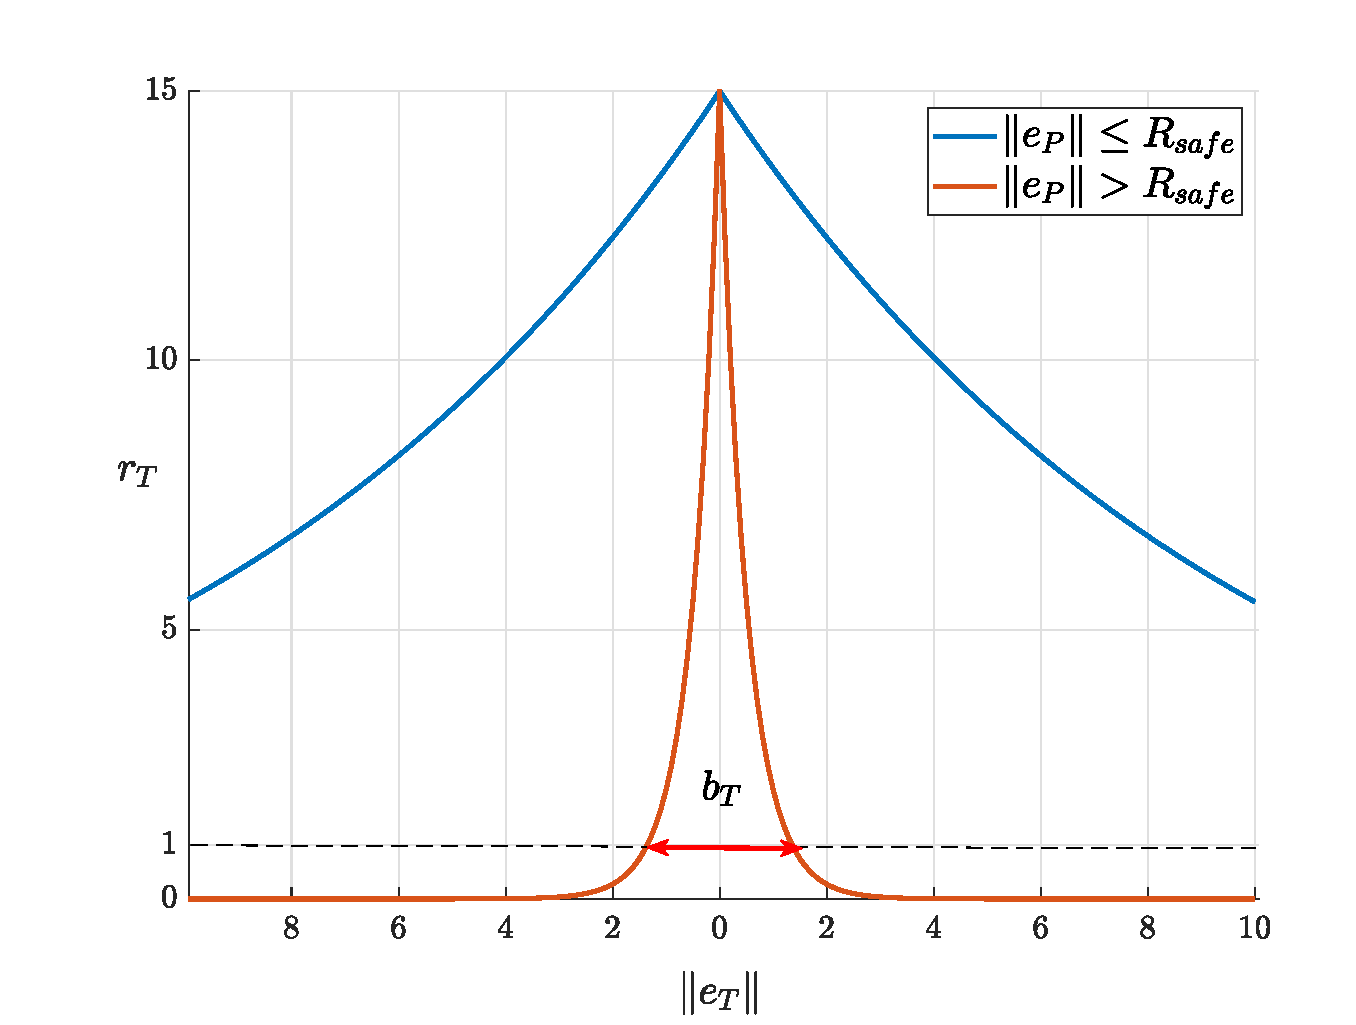
\includegraphics[scale=0.5]{figure/Part2/Chapter5/Images/reward_trajectory_final.eps}
	\caption{Trajectory reward function term.}
	\label{fig:traj_rew}
\end{figure} 

A similar approach is used to define the reward function term for the pedestrian collision avoidance, In particular, we introduce the following exponential function (see Fig.~\ref{fig:ped_rew})
\begin{equation}
	r_P (s) = 
	p_{ \rm max} (e^{ \alpha_{P} \cdot  \| e_P \|}),
\end{equation}
where  $p_{\rm max}=-15$  is the maximum penalty in correspondence of the pedestrian position and $\alpha_{P}$ is a constant defined as follows
\begin{equation}
	\alpha_{P} =  -\frac{\ln\frac{p*}{p_{\rm max}}}{b_P}. \quad 
\end{equation}

Like the previous term,  $b_{P}$ corresponds to all the relative distance values $e_P$ to the pedestrian  with $r_P \le p^*$ (in our case $p^*=1$ and $b_P = \SI{5.5}{\metre}$). As shown in Fig.~\ref{fig:ped_rew}, the pedestrian reward term is only activated when $\|e_P\| \le R_{\rm safe}$.
%is a conventional boundary on pedestrian distance for a fixed penalty $r_P(s)=p*$ and is depicted in Fig. \ref{fig:ped_rew} for $p*=-1$. Pedestrian contribution to total reward is considered only for $\|e_P\|<R_{safe}$
Both trajectory and pedestrian reward term parameters are carefully chosen in order to assure an appropriate reward function shape in the proximity of the pedestrian position as shown in Fig.~\ref{fig:traj_rew_3D}, where the maximum reward values are placed at the border of the pedestrian safe zone. 

\begin{figure}[ht]
	\centering
	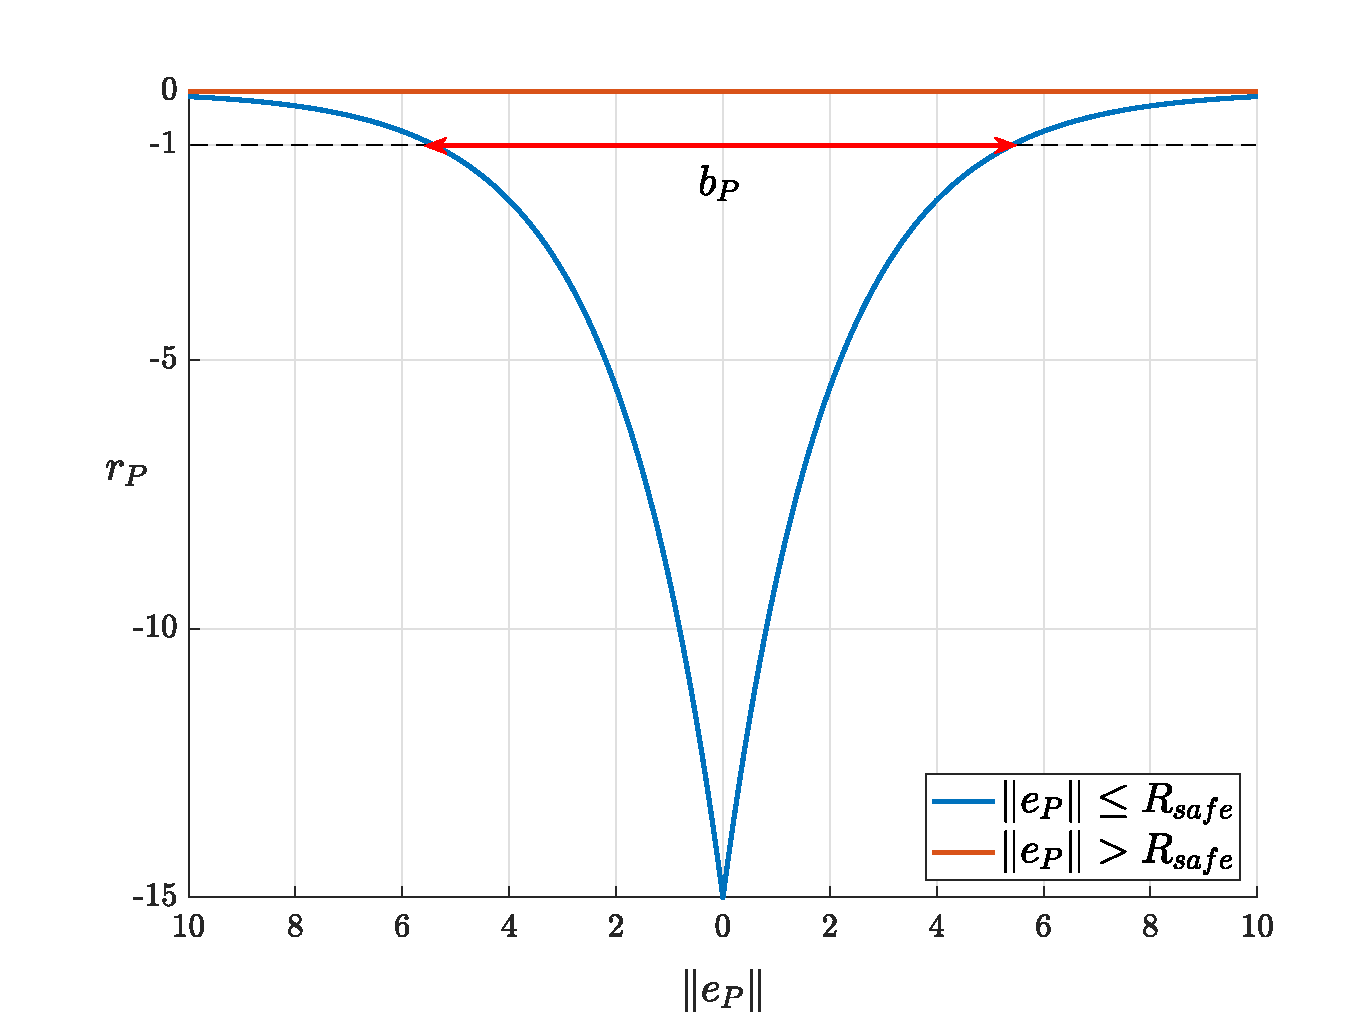
\includegraphics[scale=0.5]{figure/Part2/Chapter5/Images/Reward_pedestrian_final.eps}
	\caption{Pedestrian reward function term.}
	\label{fig:ped_rew}
\end{figure}
\begin{figure}[ht]
	\centering
	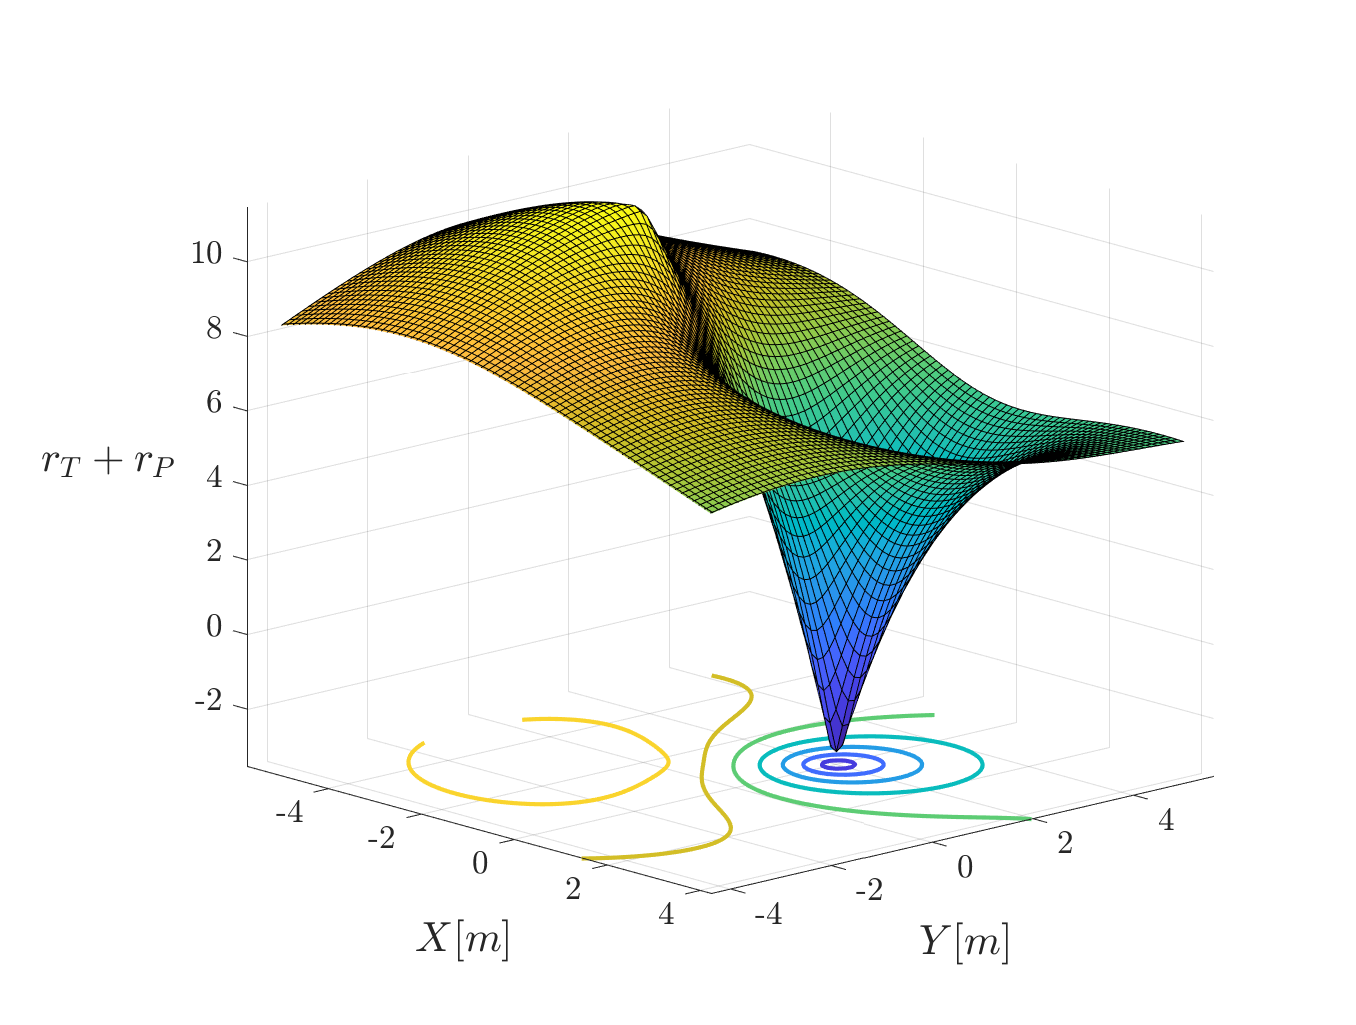
\includegraphics[scale=0.5]{figure/Part2/Chapter5/Images/Total_3D_reward.eps}
	\caption{Combination of the trajectory and pedestrian reward function terms.}
	\label{fig:traj_rew_3D}
\end{figure}


The third reward function term is linked to the selected actions 
\begin{equation}
	r_{\rm act}(s) = - \alpha_a \cdot (\| a_t-a_{t-1} \|^2 ), \\
\end{equation} 
where $\alpha_a = 10$ is the weight parameter for the control action. It aims at endorsing smooth variations of the control actions between two consecutive time slots.
%where $a$ and $a_{-1}$ represent the actual action taken and the previous one taken at the previous time step.

Two further reward terms are added to strengthen the learning process. In particular, the training episode is stopped  whenever a predetermined distance from the reference trajectory $E_{\rm max}$ is reached or the pedestrian stopping zone is entered. The following two terms are defined 
\begin{equation}
	r_{{\rm end}_P(s)}=\begin{cases}p_{P} & \text{if } e_P \leq R_{ \rm stop}, \\ 0, & \text{otherwise},
	\end{cases} 
\end{equation}
\begin{equation}
	r_{{\rm end}_T}(s)=\begin{cases} p_T & \text{if } e_{T} > E_{\rm max},  \\ 0, & \text{otherwise}. 
	\end{cases} 
\end{equation}
We set the following values: $p_{P}=p_{T}=-50$, $R_{\rm stop}=\SI{1}{\metre}$, and $E_{\rm max}=\SI{15}{\metre}$. To sum up, the complete reward function is given by the following expression
\begin{equation}
	\begin{aligned}
		r(s,a)=r_{{T}}(s)+ r_{P}(s) + r_{{\rm end}_P}(s) + r_{{\rm end}_T}(s) +  r_{\rm act}(a).
	\end{aligned}
\end{equation}
\label{sub_sec:3-e}


%\color{blue}
%Moreover to ensure safety a circle safe area with radius $R_{safe}= \SI{1}{\metre}$ is created around the pedestrian position. This abstraction is exploited in the reward shaping phase as  reported in subsection \ref{subsec:reward_shaping}.

%A stop condition is raised when the vehicle enters inside a circumference of radius $R_{safe}=\SI{1}{\metre}$. This early stopping helps the agent to improve the learning of pedestrian avoidance.



\section{Numerical simulations and results}
\label{sec:Results and conclusions}
In this section, we discuss the training process of the DDPG based agent previously described, and then we show the performance achieved by the resulting trained agent.

As expected, the training process  was influenced by three main factors: (i) the architecture of the actor and the critic neural networks (along with the values assigned to their hyper-parameters); (ii) the DDPG algorithm configuration parameters (e.g., the size of the  mini-batch $N_{\rm batch}$); the reward function definition.
%(e.g., the number of , a, see the paragraph \ref{sub_sec:3-d}.
%The choice of the actor and critic neural network hyper-parameters, see the paragraph \ref{sub_sec:3-d}.
%The reward function definition, see the paragraph %\ref{subsec:reward_shaping}.
For instance, a small mini-batch of samples  did not allow exploring the state/action space in an efficient way. In such a case, both the quality and the speed of the overall learning process were affected. Such issues were also observed when we defined and shaped the reward function. Indeed, the reward function presented in the paragraph~\ref{sub_sec:3-e} was the result of an engineering effort supported by a trial and error approach.
%resulted in a slow learning process. thus the network parameters are updated in a less precise way and the overall learning process slows down. %The decay rate $\tau_{\rm rate}$ has to be set in a proper way, so that the agent can also exploit what is has already experienced. 
%The most influential hyper-parameters  are the size of the  mini-batch $N_{\rm batch}$ and the decay rate $\tau_{ \rm rate}$ of the noise variance for the selected action $a_t$. Indeed,a small mini-batch of samples $N_{\rm batch}$ does not allow exploring the state/action space in an efficient way, thus the network parameters are updated in a less precise way and the overall learning process slows down. The decay rate $\tau_{\rm rate}$ has to be set in a proper way, so that the agent can also exploit what is has already experienced. 
%overall learning process can benefit from the exploit the of the noise variance, on the other hand, if not properly chosen may cause for the noise to affect excessively the action even when the actor's neural network has already understood a good behaviour. 
%The shape of the reward function  can considerably affect both the quality and the speed of the learning process. For instance, the reward functions shown in Fig. \ref{fig:traj_rew} and Fig. \ref{fig:ped_rew} have a very high derivative near the zero error. As a consequence, the agent can determine its correct behaviour more quickly.
%presented in the section \ref{sub_sec:3-e} is characterised by the fact that the limit of the derivative in correspondence of zero error is very high (ideally infinite) which means that small variations around the zero error determine abrupt drops in the reward, allowing the agent to  better understand the correct behaviour in less time. 

The training process was carried out for $N_{\rm ep}=6500$ episodes. 
%\st{where $N_{\rm ep}>N_{\rm noise}$. It was noted that, even when the noise added to the action was negligible, the randomness used for the mini-batch of transitions led to an improvement in the agent performance.} 
In addition, we set the sampling time  $T_s$ to $\SI{0.05}{\sec}$, the maximum time of each episode $T_{\rm sim}$  to $\SI{5}{\sec}$, and the discount factor $\gamma$ to $0.99$.
%of the tuple space sampling determines an improvement in the agent's performance.  
The outcome of the training process is shown in Fig.~\ref{fig:training_result}, where the moving mean value and the moving standard deviation of the total reward computed over the last $N_{\rm av}=20$ episodes are plotted. At the beginning of the training phase, the agent learnt to follow quickly the reference trajectory up to the beginning of the  pedestrian crosswalk area (thanks to  the exploration capabilities of the DDPG algorithm~\cite{DDPG}). After being stuck for a short period, the learning process continued, but more slowly. In this phase, we also observed increasing standard deviation values of the total reward (mainly due to the occurrence of pedestrian hits within the crosswalk area). At the end, the total reward mean value stabilised, while the related standard deviation decreased significantly. In particular, the agent learnt to avoid the pedestrian, and the residual standard deviation was only due to the distance of the vehicle from the reference trajectory. We also observed that the agent learnt to follow the reference trajectory beyond the pedestrian crosswalk area.

\begin{figure}
	\centering
	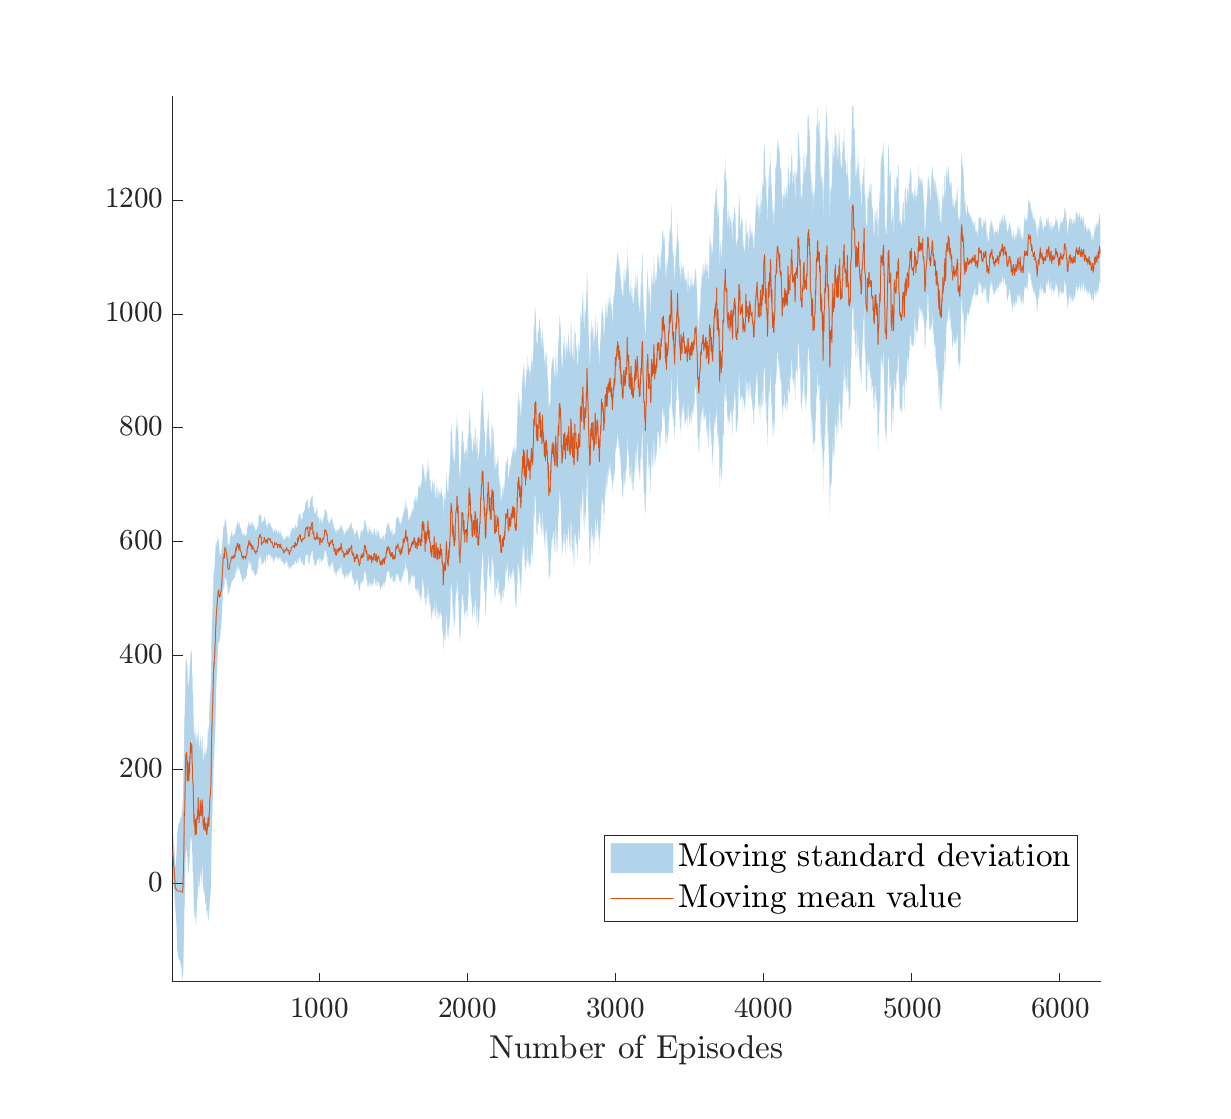
\includegraphics[scale=0.75]{figure/Part2/Chapter5/Images/std_plot.eps} 
	\caption{Moving mean value and standard deviation of the total reward during the training process.}
	\label{fig:training_result}
\end{figure}
%the blue line represents the total reward of each episode, the red line is the moving average total reward over the last $N_{\rm av}=20$ episodes, and the yellow line is the critic estimate $Q_0$ of the discounted long-term total reward at the beginning  of each episode. It is possible to distinguish four main portions in the training process as highlighted in Fig. \ref{fig:training_result} : (i) the first one in which the total reward for each episode is approximately zero since the agent explores the state space with pure random actions; (ii) the second one in which there is an improvement in the total reward thanks to the fact that the agent is able to follow the reference trajectory up to the beginning of the  pedestrian crosswalk area; (iii)  the third one characterized by slow improvement and high variance for the total reward (due to the occurrence of pedestrian hits within the crosswalk area); (iv) the fourth one where the total reward values stabilise since the agent handles more properly all the various pedestrian crossing directions, besides tracking the reference trajectory. %characterized by lowest variance and highest mean reward. We can also notice how $Q_0$ slowly converges to the experienced average total reward at the end of the training process.



\begin{figure}
	\centering
	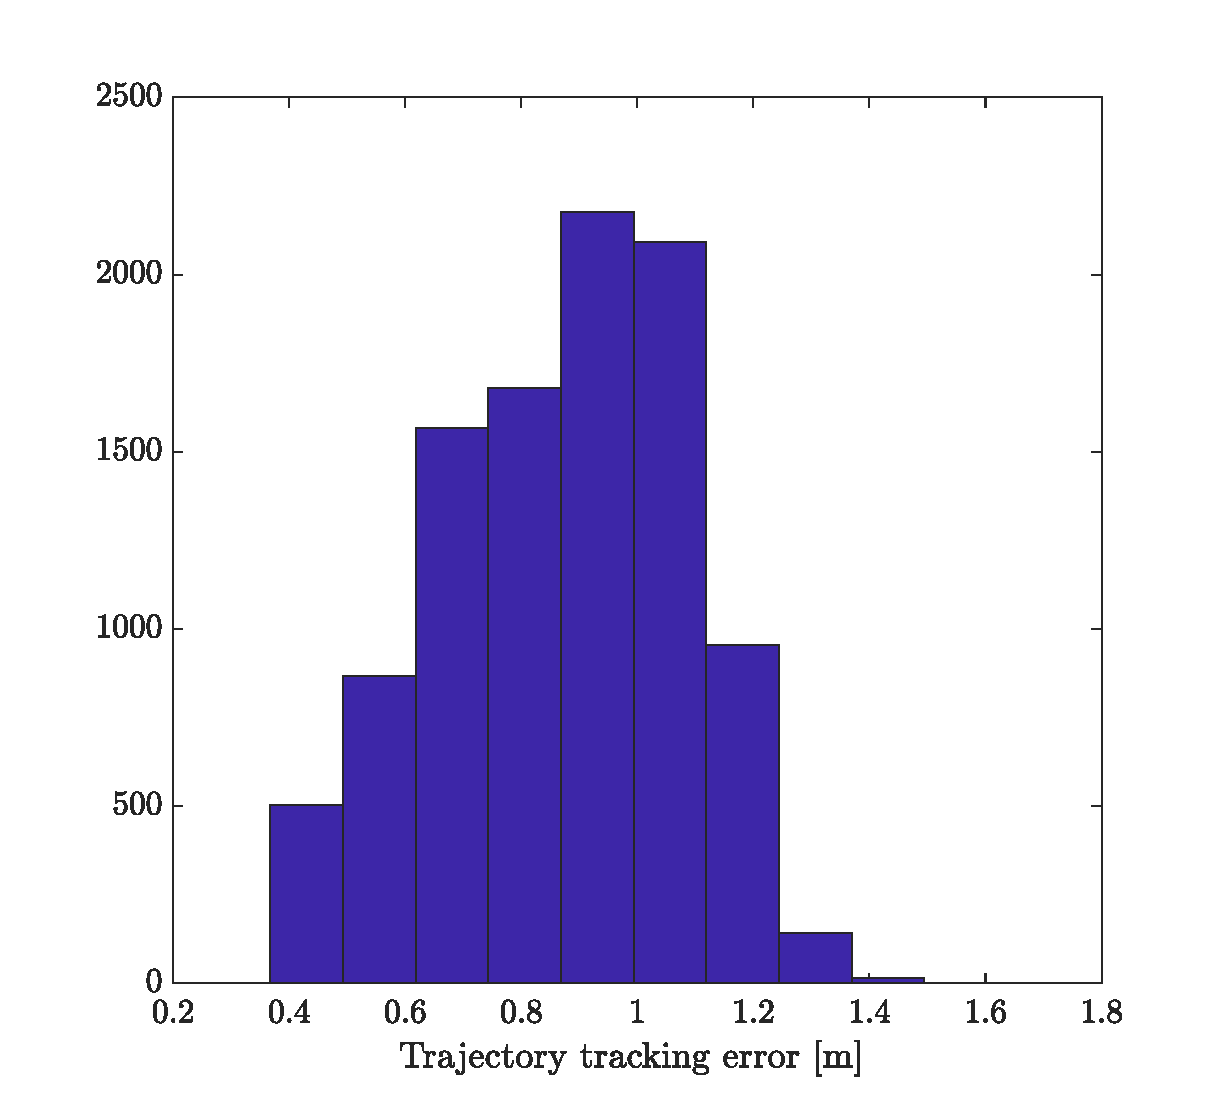
\includegraphics[scale=0.4]{figure/Part2/Chapter5/Images/err_traj.eps} 
	\caption{Maximum trajectory tracking error distribution.}
	\label{fig:episodetest}
\end{figure}


\begin{figure}
	\centering
	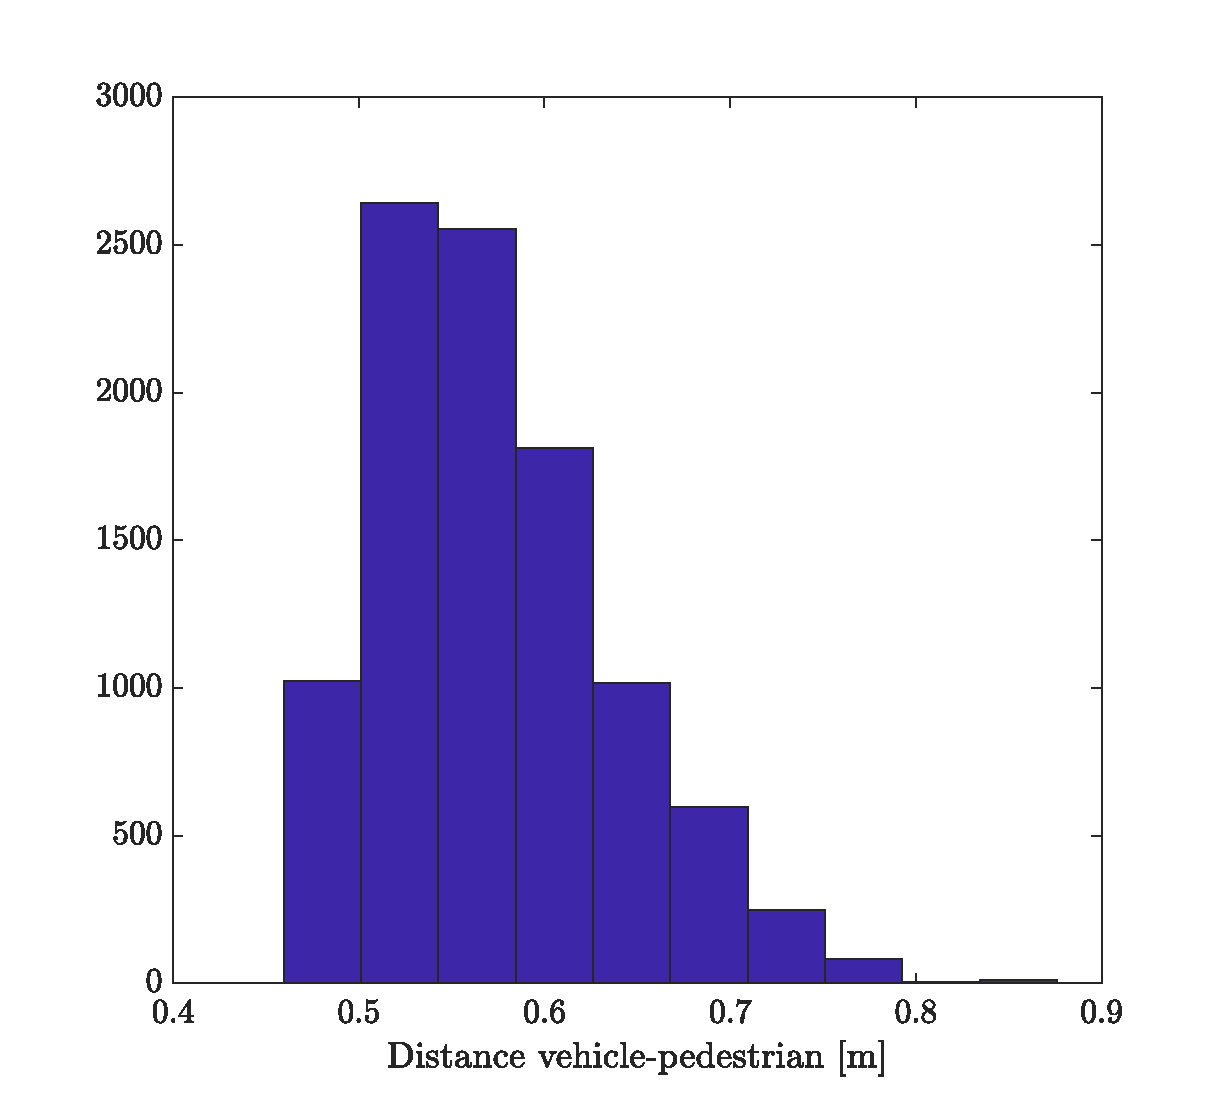
\includegraphics[scale=0.4]{figure/Part2/Chapter5/Images/err_ped_estrian.eps}
	\caption{Minimum vehicle-pedestrian distance distribution.}
	\label{fig:errorepisode}
\end{figure}

After the training phase, we tested our agent for $N_{\rm test} = 10000$ episodes, in which we observed zero pedestrian hits and adequate trajectory tracking performance. Fig.~\ref{fig:episodetest} shows the distribution of the maximum trajectory tracking error, while Fig.~\ref{fig:errorepisode} plots the distribution of the minimum vehicle-pedestrian distance.

%\color{blue}
%@Luigi: nella figura 12, una label dorebbe essere $e_{\psi}$.
%\color{black}

%\color{blue}
%Conviene in questo paragrafo indicare il valore dei parametri usato nelle simulazioni: ad esempio,
%$\sigma_{radar}= \SI{0.2}{m}$, $t_0$, $t_f$, $\sigma_x$, $\sigma_y$, $c_l$, $r_l$, $b$. Da discutere.
%\color{black}

\newpage
\section{Chapter Summary}


In conclusion, the implementation of the Deep Deterministic Policy Gradient (DDPG) algorithm for pedestrian collision avoidance in autonomous vehicles has showcased substantial potential in enhancing urban navigation safety. Through detailed numerical analysis, the algorithm demonstrated a commendable capability in reducing collision risks with pedestrians, a critical aspect of autonomous vehicle deployment in densely populated areas. The numerical results underline the algorithm's effectiveness, showing marked improvements in decision-making accuracy under various simulated urban scenarios. However, it's the inherent adaptability and learning efficiency of the DDPG algorithm that stand out, suggesting that with ongoing refinement, its application could lead to even safer and more precise autonomous driving solutions. By leveraging the strengths and addressing the limitations identified in this study, the DDPG algorithm can significantly contribute to the evolution of autonomous driving technologies, ensuring a safer coexistence between autonomous vehicles and urban pedestrians.

\chapter{A Machine Learning-Control Approach for Cybersecurity}
\label{Chapter:4}

% *** HERE STARTS THE GLOSSARY ENTRIES DEFINITION ***
% \newabbreviation{tag}{displayed acronym}{description/long name}
% \newabbreviation{}{}{}


This chapter introduces a sophisticated defense and mitigation control scheme designed to protect autonomous vehicles  during overtaking maneuvers from cyber-attacks, including Replay Attacks and Denial of Service attacks. The proposed Informative Model Predictive Scheme  architecture aims to detect and mitigate these attacks, thereby preserving the safety and integrity of AV control systems. The scheme leverages Machine Learning for attack detection, employing a Constrained Support Vector Machine classifier informed by Nonlinear Model Predictive Control data to distinguish between normal operation and various attack scenarios effectively. This approach is innovative in its adaptability to time-varying or nonlinear dynamics and its ability to implement countermeasures dynamically, showcasing a novel direction in enhancing vehicular cybersecurity. Through simulation and analysis, this chapter seeks to underline the effectiveness of the I-MPS in ensuring the safe and reliable operation of autonomous vehicles in the face of increasingly sophisticated cyber threats.

\newpage


\section{Control Strategy Architecture and Problem Formulation}
\label{sec:second}
%
We consider the~\gls{av} control architecture, depicted in Fig.~\ref{fig:architecture_attacker}, consisting on a trajectory planner which computes a high-level plan for the incoming overtaking, the proposed~\gls{imps} which is in charge of tracking the plan provided by trajectory planner, the sensory system which is responsible of providing relevant information to the on-board systems regarding the vehicle's velocity, position, acceleration and heading and  an \gls{ekf} which is in charge of filtering out the measurement noise from the measurements coming from the upstream sensory system. We further assume: (i) no model mismatch between the model used by the \gls{imps} and the mismatch for the vehicle's dynamics and (ii) that a hacker can inject \gls{ra} or \gls{dos} attacks by accessing the vehicle's CAN gateway (e.g., through Bluetooth, radio data, telematics)~\cite{bozdal2020evaluation}. 



\begin{figure}[ht]
	\centering
	
		\tikzset{every picture/.style={line width=0.9pt}} %set default line width to 0.75pt        
		\begin{tikzpicture}[x=0.75pt,y=0.75pt,yscale=-1.4,xscale=1.4]
		%uncomment if require: \path (0,300); %set diagram left start at 0, and has height of 300
		
		
		\fill[gray!30!white] (10,50) rectangle (230,140);
		\fill[gray!30!white] (10,195) rectangle (330,130);
		\node[] at (50,160) {AV control  };
		\node[] at (50,174) {architecture};
		%Shape: Rectangle [id:dp6121517022672165] 
		\draw   (19,59) -- (94.3,59) -- (94.3,108.46) -- (19,108.46) -- cycle ;
		%Shape: Rectangle [id:dp958930299715433] 
		\draw   (131.96,59) -- (207.26,59) -- (207.26,108.46) -- (131.96,108.46) -- cycle ;
		%Shape: Rectangle [id:dp44779293427709854] 
		\draw   (131.96,141.43) -- (207.26,141.43) -- (207.26,190.89) -- (131.96,190.89) -- cycle ;
		%Shape: Rectangle [id:dp5634290255034515] 
		\draw   (244.91,59) -- (320.22,59) -- (320.22,108.46) -- (244.91,108.46) -- cycle ;
		%Shape: Rectangle [id:dp5757397298802769] 
		\draw   (244.91,141.43) -- (320.22,141.43) -- (320.22,190.89) -- (244.91,190.89) -- cycle ;
		%Straight Lines [id:da9864178721017116] 
		\draw    (94.3,83.73) -- (129.96,83.73) ;
		\draw [shift={(131.96,83.73)}, rotate = 180] [color={rgb, 255:red, 0; green, 0; blue, 0 }  ][line width=0.75]    (10.93,-3.29) .. controls (6.95,-1.4) and (3.31,-0.3) .. (0,0) .. controls (3.31,0.3) and (6.95,1.4) .. (10.93,3.29)   ;
		%Straight Lines [id:da09220870807386605] 
		\draw    (207.26,83.73) -- (243.54,84.51) ;
		\draw [shift={(245.54,84.55)}, rotate = 181.23] [color={rgb, 255:red, 0; green, 0; blue, 0 }  ][line width=0.75]    (10.93,-3.29) .. controls (6.95,-1.4) and (3.31,-0.3) .. (0,0) .. controls (3.31,0.3) and (6.95,1.4) .. (10.93,3.29)   ;
		%Straight Lines [id:da35189222289389144] 
		\draw    (244.91,166.16) -- (209.26,166.16) ;
		\draw [shift={(207.26,166.16)}, rotate = 360] [color={rgb, 255:red, 0; green, 0; blue, 0 }  ][line width=0.75]    (10.93,-3.29) .. controls (6.95,-1.4) and (3.31,-0.3) .. (0,0) .. controls (3.31,0.3) and (6.95,1.4) .. (10.93,3.29)   ;
		%Straight Lines [id:da8394517684121314] 
		\draw    (320.22,83.73) -- (339.05,83.73) ;
		%Straight Lines [id:da04036512434087469] 
		\draw    (339.05,83.73) -- (339.05,166.16) ;
		%Straight Lines [id:da37873235038513076] 
		\draw    (320.22,166.16) -- (339.05,166.16) ;
		%Straight Lines [id:da23549189407989646] 
		\draw    (169.61,141.43) -- (169.61,110.46) ;
		\draw [shift={(169.61,108.46)}, rotate = 450] [color={rgb, 255:red, 0; green, 0; blue, 0 }  ][line width=0.75]    (10.93,-3.29) .. controls (6.95,-1.4) and (3.31,-0.3) .. (0,0) .. controls (3.31,0.3) and (6.95,1.4) .. (10.93,3.29)   ;
		%Image [id:dp6840101759405377] 
		\draw (226.59,214.03) node  {\includegraphics[width=19.3pt,height=26.81pt]{figure/Part2/Chapter6/Figures/cyber_attacker.jpg}};
		%Straight Lines [id:da35054905401151815] 
		\draw [color={rgb, 255:red, 208; green, 2; blue, 27 }  ,draw opacity=1 ]   (225.96,196.69) -- (226.11,169.43) ;
		\draw [shift={(226.12,167.43)}, rotate = 450.31] [color={rgb, 255:red, 208; green, 2; blue, 27 }  ,draw opacity=1 ][line width=0.75]    (10.93,-3.29) .. controls (6.95,-1.4) and (3.31,-0.3) .. (0,0) .. controls (3.31,0.3) and (6.95,1.4) .. (10.93,3.29)   ;
		
		% Text Node
		\draw (19.28,70) node [anchor=north west][inner sep=0.75pt]   [align=left] {\begin{minipage}[lt]{50.513188pt}\setlength\topsep{0pt}
			\begin{center}
			Trajectory \\Planner
			\end{center}
			
			\end{minipage}};
		% Text Node
		\draw (149,70) node [anchor=north west][inner sep=0.75pt]   [align=left] {\gls{imps} \\ Sec.~\ref{sec:I-MPS}};
		% Text Node
		\draw (254.19,63) node [anchor=north west][inner sep=0.75pt]   [align=left] {\begin{minipage}[lt]{37.855940000000004pt}\setlength\topsep{0pt}
			\begin{center}
			\vspace{0.2cm}
			Vehicle \\
			Sec.~\ref{sub_sec:vehicle_model}
			\end{center}
			
			\end{minipage}};
		% Text Node
		\draw (150,153) node [anchor=north west][inner sep=0.75pt]   [align=left] { \gls{ekf} \\ Sec.~\ref{subsec:Estimator}};
		% Text Node
		\draw (260,143) node [anchor=north west][inner sep=0.75pt]   [align=left] {Sensory \\ System \\ Sec.~\ref{sub_sec:Sensory_system}};
		% Text Node
		\draw (243,205) node [anchor=north west][inner sep=0.75pt]   [align=left] {\textcolor[rgb]{0.82,0.01,0.11}{HACKER}\\ Sec.~\ref{sub_sec:attacker_model}};
		
		
		\end{tikzpicture}

	\caption{ \gls{av} control architecture. The hacker corrupts the outputs of the sensory system.}
	\label{fig:architecture_attacker}
\end{figure}
%




\subsection{Vehicle Model}
\label{sub_sec:vehicle_model}
%
Vehicles operating in an urban environment can be modeled via a kinematic bicycle based model~\cite{bicycle_Borrelli},~\cite{Bicycle_model_2}. In such model, the wheels do not slip at their contact point with the ground since both the velocity and the acceleration values are assumed to be low. Furthermore,  we assume that the vehicle is a front wheel steering vehicle.

Thus, the vehicle dynamics are given by~\cite{bicycle_Borrelli}
%
\begin{subequations}
	\label{eq:vehicmodel}
	\begin{align}
		\dot{x} &= v \cos \big(\psi+\beta\big),\\
		\dot{y}  &= v \sin \big(\psi+\beta\big),\\
		\dot{\psi}  &= \frac{v}{l_{r}} \sin \beta,\\
		\dot{v}  &= a,
	\end{align}
\end{subequations}
% Se usi il commento non hai bisogno di istanziare un \noindent. Troppi comandi non sono raccomandabili perché in alcune condizioni potrebbero scemunire il compilatore. Col commento ottieni il risultato di segmentare il testo per, deduco, migliorare la leggibilità senza generare indentazioni tipiche di un nuovo capoverso.
where $x$ and $y$ are the coordinates of the vehicle mass-center in an inertial frame, $\psi$ is the heading angle of the vehicle mass-center, $v$ is the velocity of the vehicle mass-center, $a$ is the mass-center acceleration, $\beta =\arctan\Big(l_{r}\tan \delta_f\slash(l_{f}+l_{r}) \Big)$ is the side slip angle of the vehicle, and $l_f$ and $l_r$ are the distances of the front and rear axles from the mass-center, respectively, $\delta_f$  and  $a$ the steering angle and acceleration, respectively. 

In what follows, $\zeta=\begin{bmatrix}x & y & \psi & v\end{bmatrix}^\top \in \mathbb{R}^{4 } $ and \mbox{$u=\begin{bmatrix}\delta_f & a\end{bmatrix}^\top \in \mathbb{R}^{2 }$ } will be used to indicate the state and the input vectors of the system, respectively.

\subsection{Sensory System}
\label{sub_sec:Sensory_system}
%
The state measurements supplied by the Sensory System module are subject to additive noise and are modeled as 
% se lasci una riga poi nel pdf c'è uno spazio troppo grande
\begin{equation}\label{eq:sensor_measurements}
	\zeta_m = \zeta + \eta,
\end{equation}
%	
where $\zeta_m=\begin{bmatrix} x_m & y_m & \psi_m & v_m \end{bmatrix}^\top$ and $\eta=\begin{bmatrix} \eta_x & \eta_y & \eta_\psi & \eta_v \end{bmatrix}^\top$, with $\eta_x$, $\eta_y$, $\eta_{\psi}$ and $\eta_v$ being zero mean, white Gaussian noises. The state measurements vector $\zeta_m$ is the whole knowledge accessible by the hacker. 

\subsection{Hacker Model}
\label{sub_sec:attacker_model}
%
In this subsection we define how a hacker can corrupt the measurements, as depicted in Fig.~\ref{fig:architecture_attacker}. For both attacks, $t_a$ and $T_d$ will indicate the time at which an attack starts and its duration, respectively.
%
\paragraph{Replay Attacks}
\glspl{ra} consist of a recording and a replay phase. During the recording phase, the hacker stores the past measurements, which in the replay phase are injected into the system. The \gls{ra} model is given by~\cite{teixeira2015secure}
%
\begin{equation} \label{eq:replay_model}
	\zeta^{\rm RA}_{m}(t) = \begin{cases}  \zeta_m(t-T_d), & \mbox{if } t \in \big[t_a,t_a+ T_d\big], \\ \zeta_m(t), & \mbox{otherwise}.  \end{cases}
\end{equation} 
%	
with the recording taking place in the time interval~\mbox{$\big[t_a-T_d,t_a\big]$}.
%
\paragraph{Denial of Service Attacks}
In this case, the hacker interrupts the data stream between the Sensory System and the \gls{ekf}. In real vehicles the \gls{ecu}, where the Controller block is implemented, typically holds the last useful data in the local memory which is then used in place of the expected new ones when they are not available. The model for \gls{dos} attacks is~\cite{schenato2009zero}
%
\begin{equation}
	\label{eq:Dos_model}
	\zeta^{\rm DoS}_{m}(t)=%
	\begin{cases}
		\zeta_m\big(t\big)\big|_{t=t_a}, & \mbox{if } t \in \big[t_a,t_a+T_d\big], \\ \zeta_m(t), & \mbox{otherwise}.
	\end{cases}
\end{equation} 
%
That is, the effect of the \gls{dos} attack consists in resending the sensor measured at the time $t=t_a$ during the time interval $\big[t_a,t_a+T_d\big]$.
\subsection{\gls{ekf}}
\label{subsec:Estimator}
%
In this work, the \gls{ekf}~\cite{EKF_3} provides the estimates $\hat\zeta$ of the vehicle's dynamics to the \gls{imps} block. Although the use of this estimator could improve the detectability of a cyber-attack~\cite{ekf_1_attack}, in the case under investigation, it is in charge only to provide the state estimation to the \gls{nmpc}.




%%% END SECTION ============================================================

%%% START SECTION ==========================================================

\section{I-MPS}
\label{sec:I-MPS}
%
Fig.~\ref{fig:I-NMPC} shows the proposed \gls{imps}. It includes three interconnected modules: the Detector, the Mitigator and an \gls{nmpc}. However, the architecture and the deriving scheme are general enough so as to allow other types of Model Based Controller such as, e.g., LTI-MPC, \gls{ltvmpc}, \gls{lpvmpc}. A discrete-time setting is assumed with $k$ being the discrete-time variable and $T_s$ being the sampling time such that $t=kT_s$.
%
\begin{figure}[H]
	\centering
	


\tikzset{every picture/.style={line width=0.75pt}} %set default line width to 0.75pt        

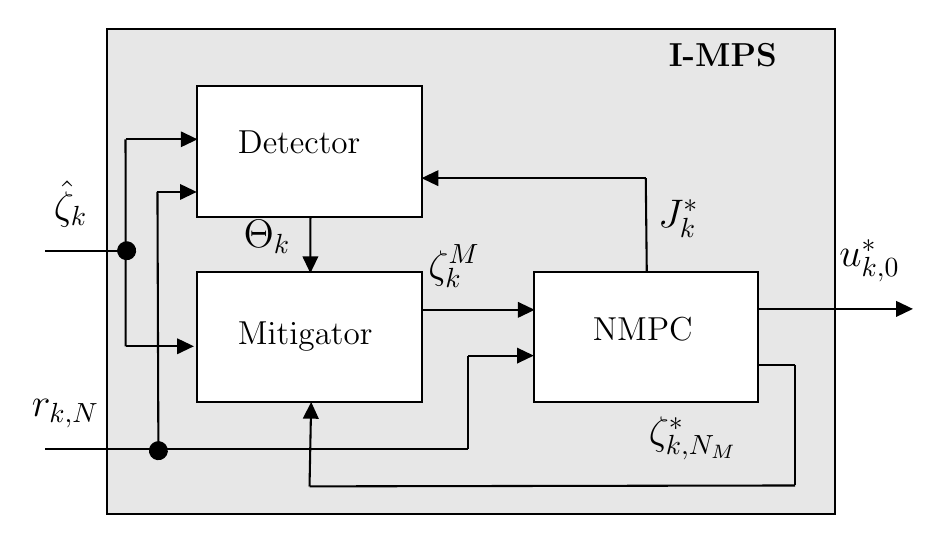
\begin{tikzpicture}[x=0.75pt,y=0.75pt,yscale=-0.9,xscale=0.9]
%uncomment if require: \path (0,300); %set diagram left start at 0, and has height of 300

%Shape: Rectangle [id:dp07321239801052792] 
\draw  [color={rgb, 255:red, 0; green, 0; blue, 0 }  ,draw opacity=1 ][fill={rgb, 255:red, 231; green, 231; blue, 231 }  ,fill opacity=1 ] (121.5,30) -- (511.5,30) -- (511.5,290) -- (121.5,290) -- cycle ;
%Shape: Rectangle [id:dp1563881976892849] 
\draw  [fill={rgb, 255:red, 255; green, 255; blue, 255 }  ,fill opacity=1 ] (170,160) -- (290,160) -- (290,230) -- (170,230) -- cycle ;
%Shape: Rectangle [id:dp978555336465935] 
\draw  [fill={rgb, 255:red, 255; green, 255; blue, 255 }  ,fill opacity=1 ] (170,60.67) -- (290,60.67) -- (290,130.67) -- (170,130.67) -- cycle ;
%Shape: Rectangle [id:dp6438542779108847] 
\draw  [fill={rgb, 255:red, 255; green, 255; blue, 255 }  ,fill opacity=1 ] (350,160) -- (470,160) -- (470,230) -- (350,230) -- cycle ;
%Straight Lines [id:da2661535299648963] 
\draw    (290.5,180.5) -- (347.5,180.5) ;
\draw [shift={(350.5,180.5)}, rotate = 180] [fill={rgb, 255:red, 0; green, 0; blue, 0 }  ][line width=0.08]  [draw opacity=0] (8.93,-4.29) -- (0,0) -- (8.93,4.29) -- cycle    ;
%Straight Lines [id:da9975743928269731] 
\draw    (470,180) -- (550,180) ;
\draw [shift={(553,180)}, rotate = 180] [fill={rgb, 255:red, 0; green, 0; blue, 0 }  ][line width=0.08]  [draw opacity=0] (8.93,-4.29) -- (0,0) -- (8.93,4.29) -- cycle    ;
%Straight Lines [id:da45105295619600305] 
\draw    (410,110) -- (410.55,160.67) ;
%Straight Lines [id:da31332759246635855] 
\draw    (410,110) -- (293,110) ;
\draw [shift={(290,110)}, rotate = 360] [fill={rgb, 255:red, 0; green, 0; blue, 0 }  ][line width=0.08]  [draw opacity=0] (8.93,-4.29) -- (0,0) -- (8.93,4.29) -- cycle    ;
%Straight Lines [id:da6831976187030333] 
\draw    (131.5,89.2) -- (131.55,200) ;
%Straight Lines [id:da5381627981193056] 
\draw    (131.5,89.2) -- (167,89.2) ;
\draw [shift={(170,89.2)}, rotate = 180] [fill={rgb, 255:red, 0; green, 0; blue, 0 }  ][line width=0.08]  [draw opacity=0] (8.93,-4.29) -- (0,0) -- (8.93,4.29) -- cycle    ;
%Straight Lines [id:da9898851017884422] 
\draw    (490,210) -- (490,274.52) ;
%Straight Lines [id:da424908054336965] 
\draw    (470,210) -- (490,210) ;
%Straight Lines [id:da2810640697891009] 
\draw    (230,275) -- (230.82,232.82) ;
\draw [shift={(230.88,229.82)}, rotate = 451.11] [fill={rgb, 255:red, 0; green, 0; blue, 0 }  ][line width=0.08]  [draw opacity=0] (8.93,-4.29) -- (0,0) -- (8.93,4.29) -- cycle    ;
%Straight Lines [id:da4824194165524387] 
\draw    (230,275) -- (490,274.52) ;
%Straight Lines [id:da6654648688677554] 
\draw    (230.5,130.91) -- (230.46,157.85) ;
\draw [shift={(230.45,160.85)}, rotate = 270.09000000000003] [fill={rgb, 255:red, 0; green, 0; blue, 0 }  ][line width=0.08]  [draw opacity=0] (8.93,-4.29) -- (0,0) -- (8.93,4.29) -- cycle    ;
%Shape: Circle [id:dp22585331850262147] 
\draw  [fill={rgb, 255:red, 0; green, 0; blue, 0 }  ,fill opacity=1 ] (127.76,150.09) .. controls (127.07,147.7) and (128.45,145.2) .. (130.84,144.51) .. controls (133.23,143.82) and (135.73,145.2) .. (136.42,147.59) .. controls (137.12,149.98) and (135.74,152.48) .. (133.34,153.17) .. controls (130.95,153.87) and (128.45,152.49) .. (127.76,150.09) -- cycle ;
%Straight Lines [id:da506959418744912] 
\draw    (88.55,148.84) -- (132.09,148.84) ;
%Straight Lines [id:da9298485020674954] 
\draw    (131.55,200) -- (165.05,200) ;
\draw [shift={(168.05,200)}, rotate = 180] [fill={rgb, 255:red, 0; green, 0; blue, 0 }  ][line width=0.08]  [draw opacity=0] (8.93,-4.29) -- (0,0) -- (8.93,4.29) -- cycle    ;
%Straight Lines [id:da32869903555712465] 
\draw    (88.5,255) -- (315,255) ;
%Straight Lines [id:da035880638063171544] 
\draw    (315,205) -- (315,255) ;
%Straight Lines [id:da6563089432200115] 
\draw    (315,205) -- (347,205) ;
\draw [shift={(350,205)}, rotate = 180] [fill={rgb, 255:red, 0; green, 0; blue, 0 }  ][line width=0.08]  [draw opacity=0] (8.93,-4.29) -- (0,0) -- (8.93,4.29) -- cycle    ;
%Shape: Circle [id:dp41684320512129514] 
\draw  [fill={rgb, 255:red, 0; green, 0; blue, 0 }  ,fill opacity=1 ] (144.76,257.14) .. controls (144.07,254.74) and (145.45,252.24) .. (147.84,251.55) .. controls (150.23,250.86) and (152.73,252.24) .. (153.42,254.64) .. controls (154.12,257.03) and (152.74,259.53) .. (150.34,260.22) .. controls (147.95,260.91) and (145.45,259.53) .. (144.76,257.14) -- cycle ;
%Straight Lines [id:da35344859328738143] 
\draw    (148.59,117.39) -- (149.09,255.89) ;
%Straight Lines [id:da8249585929292025] 
\draw    (148.59,117.39) -- (166.59,117.39) ;
\draw [shift={(169.59,117.39)}, rotate = 180] [fill={rgb, 255:red, 0; green, 0; blue, 0 }  ][line width=0.08]  [draw opacity=0] (8.93,-4.29) -- (0,0) -- (8.93,4.29) -- cycle    ;

% Text Node
\draw (420.67,36.17) node [anchor=north west][inner sep=0.75pt]  [font=\large] [align=left] {\textbf{I-MPS}};
% Text Node
\draw (380,183) node [anchor=north west][inner sep=0.75pt]  [font=\large] [align=left] {NMPC};
% Text Node
\draw (190,83) node [anchor=north west][inner sep=0.75pt]  [font=\large] [align=left] {Detector};
% Text Node
\draw (190,185) node [anchor=north west][inner sep=0.75pt]  [font=\large] [align=left] {Mitigator};
% Text Node
\draw (79.67,227) node [anchor=north west][inner sep=0.75pt]  [font=\Large]  {$r_{k,N}$};
% Text Node
\draw (91.5,110) node [anchor=north west][inner sep=0.75pt]  [font=\Large]  {$\hat{\zeta }_{k}$};
% Text Node
\draw (292,144) node [anchor=north west][inner sep=0.75pt]  [font=\Large]  {${\zeta^{M}_{k}}$};
% Text Node
\draw (512,141) node [anchor=north west][inner sep=0.75pt]  [font=\Large]  {$u^{*}_{k,0}$};
% Text Node
\draw (415,120) node [anchor=north west][inner sep=0.75pt]  [font=\Large]  {$J^{*}_{k}$};
% Text Node
\draw (193,131) node [anchor=north west][inner sep=0.75pt]  [font=\Large]  {$\Theta _{k}$};
% Text Node
\draw (410,236.17) node [anchor=north west][inner sep=0.75pt]  [font=\Large]  {$\zeta ^{*}_{k,N_M}$};


\end{tikzpicture}
	\caption{\gls{imps} architecture.}
	\label{fig:I-NMPC}
\end{figure}
%
\subsection{NMPC for Trajectory Tracking}
\label{subsec:NMPC}
%
The \gls{nmpc} is solved at each $k$ by minimizing the cost function
\begin{align}\label{eq:J}
	\nonumber J_k=&\sum_{i=k}^{k+N}(\zeta_i-r_i)^\top L(\zeta_i-r_i)\\&+\sum_{i=k}^{k+N-1} (u_i-u_{i-1})^\top S(u_i-u_{i-1}) + u_i^\top R u_i,
\end{align}
across the prediction horizon $N$ and where \mbox{$\zeta_{i}=\begin{bmatrix} x_i & y_i & \psi_i & v_i \end{bmatrix}^\top$} is the $i$-th future state vector of the vehicle's dynamic model used by the \gls{nmpc}, $r_i$ is the $i$-th future reference provided by the trajectory planner through the sequence $r_{k,N} = \big\{r_k, \ldots, r_{k+N}\big\}$, $u_i$ is the $i$-th \gls{nmpc} future outputs, and $L$, $S$ and $R$ are suitable weighting matrices of appropriate dimensions by which the control input performances are taken into account. 

The discrete-time optimization problem is solved by discretizing the continuous time model~\eqref{eq:vehicmodel} assuming a piecewise constant control $u(\tau)=u_k$, with $\tau \in \big[t_k,t_{k+1}\big[$, and then using the multiple shooting method~\cite{NMPC_1} which yields the constraint
\begin{equation}\label{eq:con_integrator}
	\zeta_{k+1}-\Xi(\zeta_k,u_k) = 0,
\end{equation}
where $\Xi(\zeta_k,u_k)$ is the $4$-th order Runge-Kutta integrator for the integration of the system dynamics over the shooting interval. Furthermore, the initial state is included as constraint into the optimization problem as follow
\begin{equation}\label{eq:con_init}
	\zeta_k -{\zeta}^M_{k}=0,
\end{equation}
where ${\zeta}^M_{k}$ is the Mitigator output.



The physical limitations of the control input regarding the  minimum  and  maximum values, $u_{\mathrm{min}}$ and $u_{\mathrm{max}}$, respectively, and slew-rates, $\dot{u}_{\mathrm{min}}$ and $\dot{u}_{\mathrm{max}}$, respectively, that the actuation system is capable of, can be taken into account as
\begin{subequations}\label{eq:con_u_tot}
	\begin{align}
		u_{\mathrm{min}} \leq u_k  \leq& u_{\mathrm{max}},\label{eq:con_u}\\
		\dot u_{\mathrm{min}} \leq \dot{u}_k \leq& \dot{u}_{\mathrm{max}}.\label{eq:con_dot_u}
	\end{align}
\end{subequations}


Ultimately, the \gls{nmpc} computes
%
\begin{argmini}|s|
	{\zeta_{k,N}, u_{k,N-1}}{\eqref{eq:J}}{}{\zeta_{k,N}^\ast, u_{k,N-1}^\ast=}
	{\label{eq:opt_probl}}{}
	\addConstraint{\eqref{eq:con_integrator}-\eqref{eq:con_u_tot},}{}
\end{argmini}
%porta nel testo $u_{-1} = u(t-T_s)$
%
where $\zeta_{k,N} =\big\{\zeta_k, \ldots, \zeta_{k+N}\big\}$ and $u_{k,N-1} = \big\{u_k, \ldots, u_{k+N-1}\big\}$. 

\subsection{Mitigator}\label{subsec:Mitigator}
The Mitigator is triggered depending to the  flag $\Theta_k \in \{0, 1\}$ (see Fig.~\ref{fig:I-NMPC}): if $\Theta_k=0$ no cyber-attack has been detected and the state estimate $\hat{\zeta}_k$ can be fed to the \gls{nmpc} at the current iteration $k$; while, if $\Theta_k=1$ a cyber-attack has been detected and a countermeasure is taken. Thus, the Mitigator implements
%
\begin{equation} \label{eq:mean_predictions}
	\zeta^M_{k} = \begin{cases} \hat{\zeta }_k & \mbox{if } \Theta_k=0, \\ \bar{\zeta}_k &  \mbox{if } \Theta_k=1,  \end{cases}
\end{equation} 
\noindent where $\hat{\zeta}_k $ is the state estimate at time-instant $k$ and
%	
\begin{equation}\label{mean_predict}
	\bar{\zeta}_k=
	\sum_{i=k-N_M}^{k-1} \frac{\zeta^\ast_{i,k}}{N_M},
\end{equation}
where $\zeta^\ast_{i,k}$ is the optimal state that was computed by the $(k-i)$-th \gls{nmpc} iteration and considered at current time $k$, $N_M \leq N$ is the number of past samples used by the Mitigator at current time $k$ and \mbox{$\bar\zeta=\begin{bmatrix} \bar x & \bar y & \bar \psi & \bar v \end{bmatrix}^\top$}.


\subsection{Detector}
\label{subsec:Detector}
%
The Detector is a \gls{csvm} classifier trained against \gls{ra} and \gls{dos} attacks. In particular, a multiclass classification problem is considered, with classes reported in Table~\ref{table:classes}.

\begin{table}[ht]
	\centering
	\begin{tabular}{ |c|c|c| } 
		\hline
		Class & Cyber-attack & Number of instances\\
		\hline
		\multirow{7}{2em}{\centering $0$\\[2.2pt] $1$\\[2.2pt]  $2$\\[2.2pt]  $3$\\[2.2pt]  $4$\\[2.2pt]  $5$\\[2.2pt]  $6$} 
		
		& No attacks & $14765$\\[1.5pt] 
		& $\big\{x_m, \; y_m\big\}_{\rm DoS}$ & $3135$ \\[1.5pt]  
		& $\big\{\psi_m,v_m\big\}_{\rm DoS}$ & $3154$ \\[1.5pt]  
		& $\big\{x_m, \; y_m\big\}_{\rm DoS} \cup \big\{\psi_m,v_m\big\}_{\rm DoS}$ & $3126$\\[1.5pt]  
		& $\big\{x_m, \; y_m\big\}_{\rm RA}$ & $1812$  \\[1.5pt]  
		& $\big\{\psi_m,v_m\big\}_{\rm RA}$ & $1708$ \\[1.5pt]  
		& $\big\{x_m, \; y_m\big\}_{\rm RA} \cup \big\{\psi_m,v_m\big\}_{\rm RA}$ & $1830$ \\[1.5pt]  
		\hline
	\end{tabular}
	\vspace{0.25 cm}
	\caption{Class definitions.}
	\label{table:classes}
\end{table}
%
The class $0$ identifies the case in which no cyber-attacks occur. The classes  $1$--$3$ and \mbox{$4$--$6$} regard \gls{ra} and \gls{dos} attack onto either part or the entire attack space. In particular, the hacker is assumed to be able to access the set $\big\{x_m, \; y_m \big\}$ of the position measurements, the set $\big\{\psi_m, \; v_m \big\}$ of the heading and velocity measurements, or the set $\big\{x_m, \; y_m \big\} \cup \big\{\psi_m, \; v_m \big\}$. The particular choice of the classes has derived by the assumption that hacker affects the ECUs of the GPS and/or pose sensors. At each $k$, three features are used for detection: the first is the error
\begin{equation}\label{eq:err}
	e_{\hat\zeta,k}=\hat\zeta_k - r_k,
\end{equation}
between the state estimates from the \gls{ekf} and the references provided by the trajectory planner, the second is the \gls{nmpc} cost function $J_k$ in~\eqref{eq:J}, the third is the vector
\begin{equation}\label{eq:kl_div}
	D^{\mathrm{KL}}_k =%
	\begin{bmatrix}
		D^{\mathrm{KL}}_k\big(\bar{E}_x \| Q_{x,k}\big)\\
		D^{\mathrm{KL}}_k\big(\bar{E}_y \| Q_{y,k}\big)\\
		D^{\mathrm{KL}}_k\big(\bar{E}_\psi \| Q_{\psi,k}\big)\\
		D^{\mathrm{KL}}_k\big(\bar{E}_v \| Q_{v,k}\big)
	\end{bmatrix},
\end{equation}
of the \gls{kl}\footnote{The \gls{kl} divergence between two probability densities $p(x)$ and $q(x)$ is defined as \begin{equation*}D_{\mathrm{KL}}(P \| Q)=\int_{-\infty}^{\infty} p(x) \log \left(\frac{p(x)}{q(x)}\right) dx.    \end{equation*}}
divergences between the estimated probability densities of $\bar E_x$, $\bar E_y$, $\bar E_\psi$ and $\bar E_v$ of $\bar e_x=\bar x - \hat x $, $\bar e_y=\bar y - \hat y$, $e_\psi =\bar \psi - \hat \psi$ and $\bar e_v=\bar v - \hat v$, respectively, under known conditions when no cyber-attack is taking place and the corresponding $Q_{x,k}$, $Q_{y,k}$, $Q_{\psi,k}$ and $Q_{v,k}$ estimated during the driving during the time window \mbox{$\big\{k-N_M,\ldots,k-1\big\}$} at the current time $k$. Here, the errors $\bar e_x$, $\bar e_y$, $\bar e_\psi$ and $\bar e_v$ are calculated the difference between $\bar \zeta$ and $\hat \zeta$ which represent the predicted state from the past and the state estimate, respectively.

\begin{figure}
	\centering
	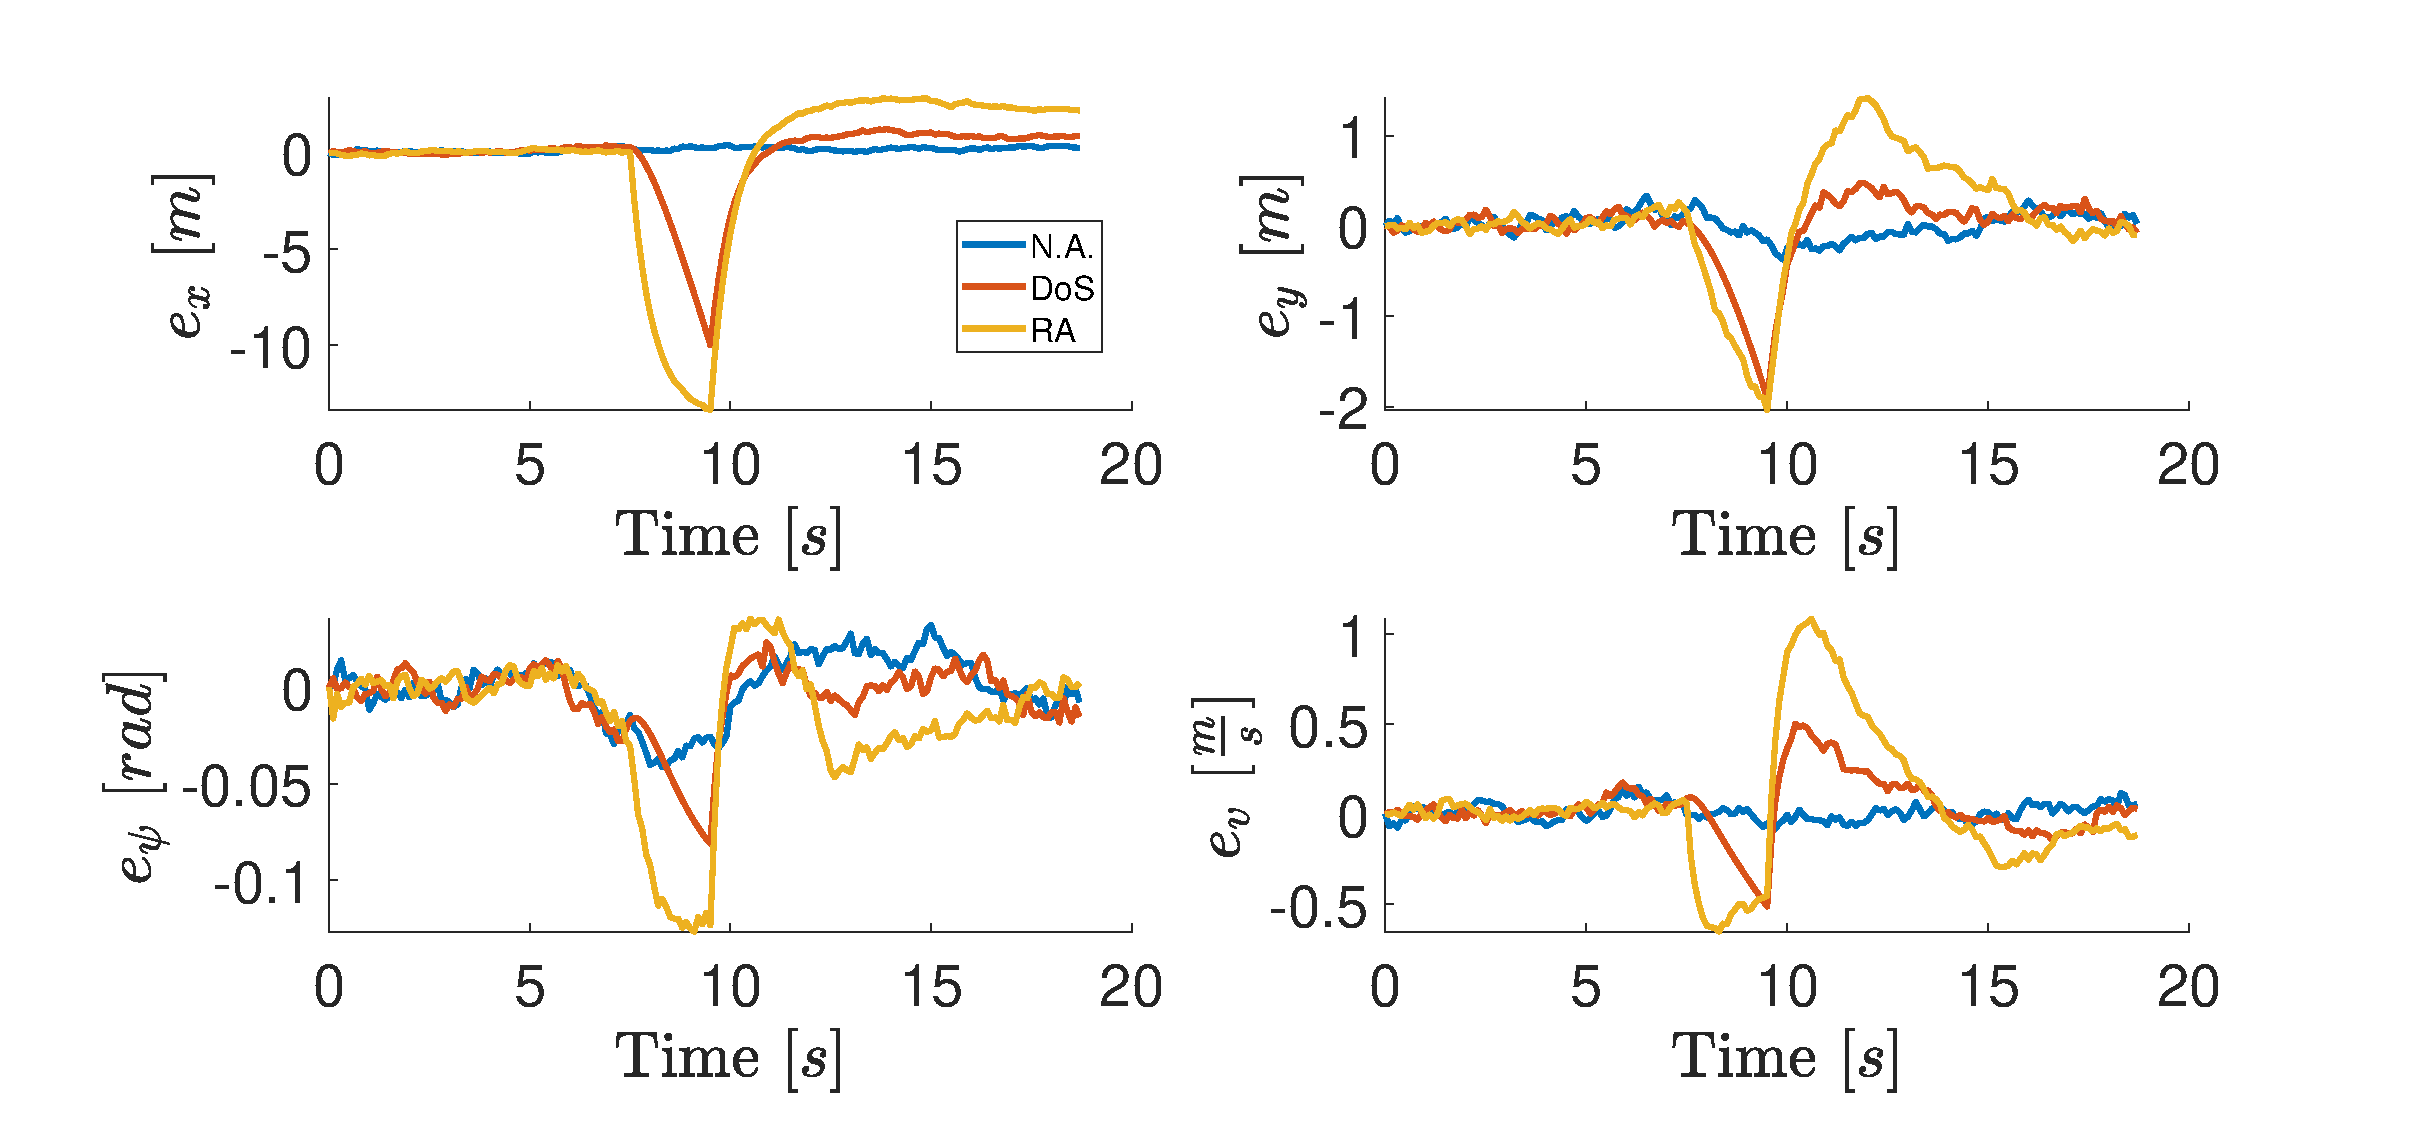
\includegraphics[scale=0.4]{figure/Part2/Chapter6/Figures/Errors_All.eps}
	\caption{Errors $e_{\zeta}$. Top-left: $e_x$. Top-right: $e_y$. Bottom-left: $e_{\psi}$. Bottom-right: $e_v$.  }
	\label{fig:gamma_error}
\end{figure}

\begin{figure}
	\centering
	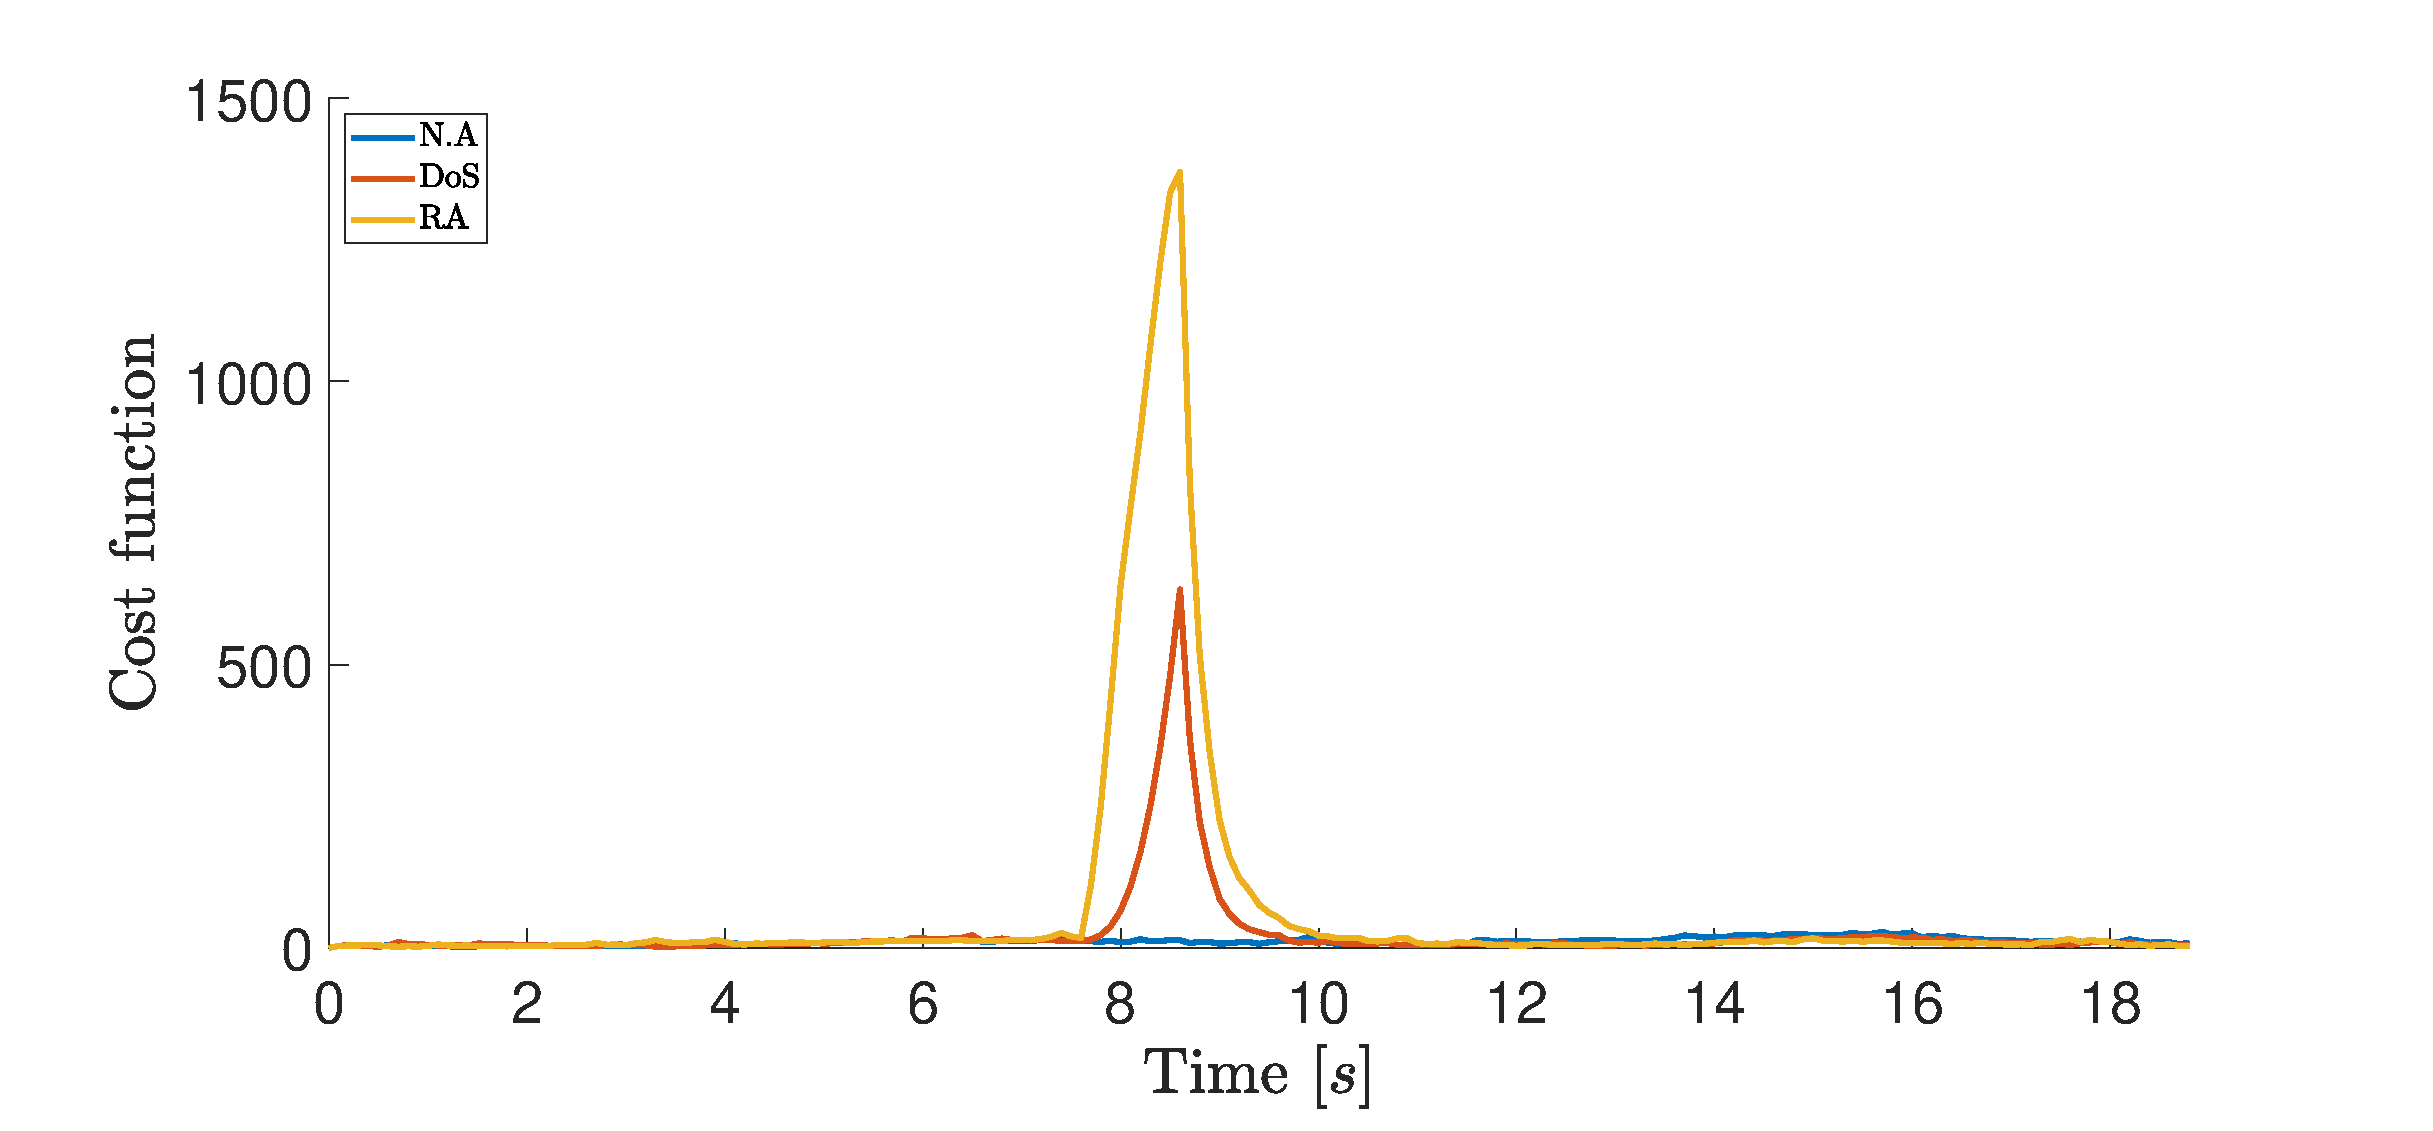
\includegraphics[scale=0.4]{figure/Part2/Chapter6/Figures/J_All.eps}
	\caption{Functional cost $J^\ast$. } 
	\label{fig:gamma_J}
\end{figure}

\begin{figure}
	\centering
	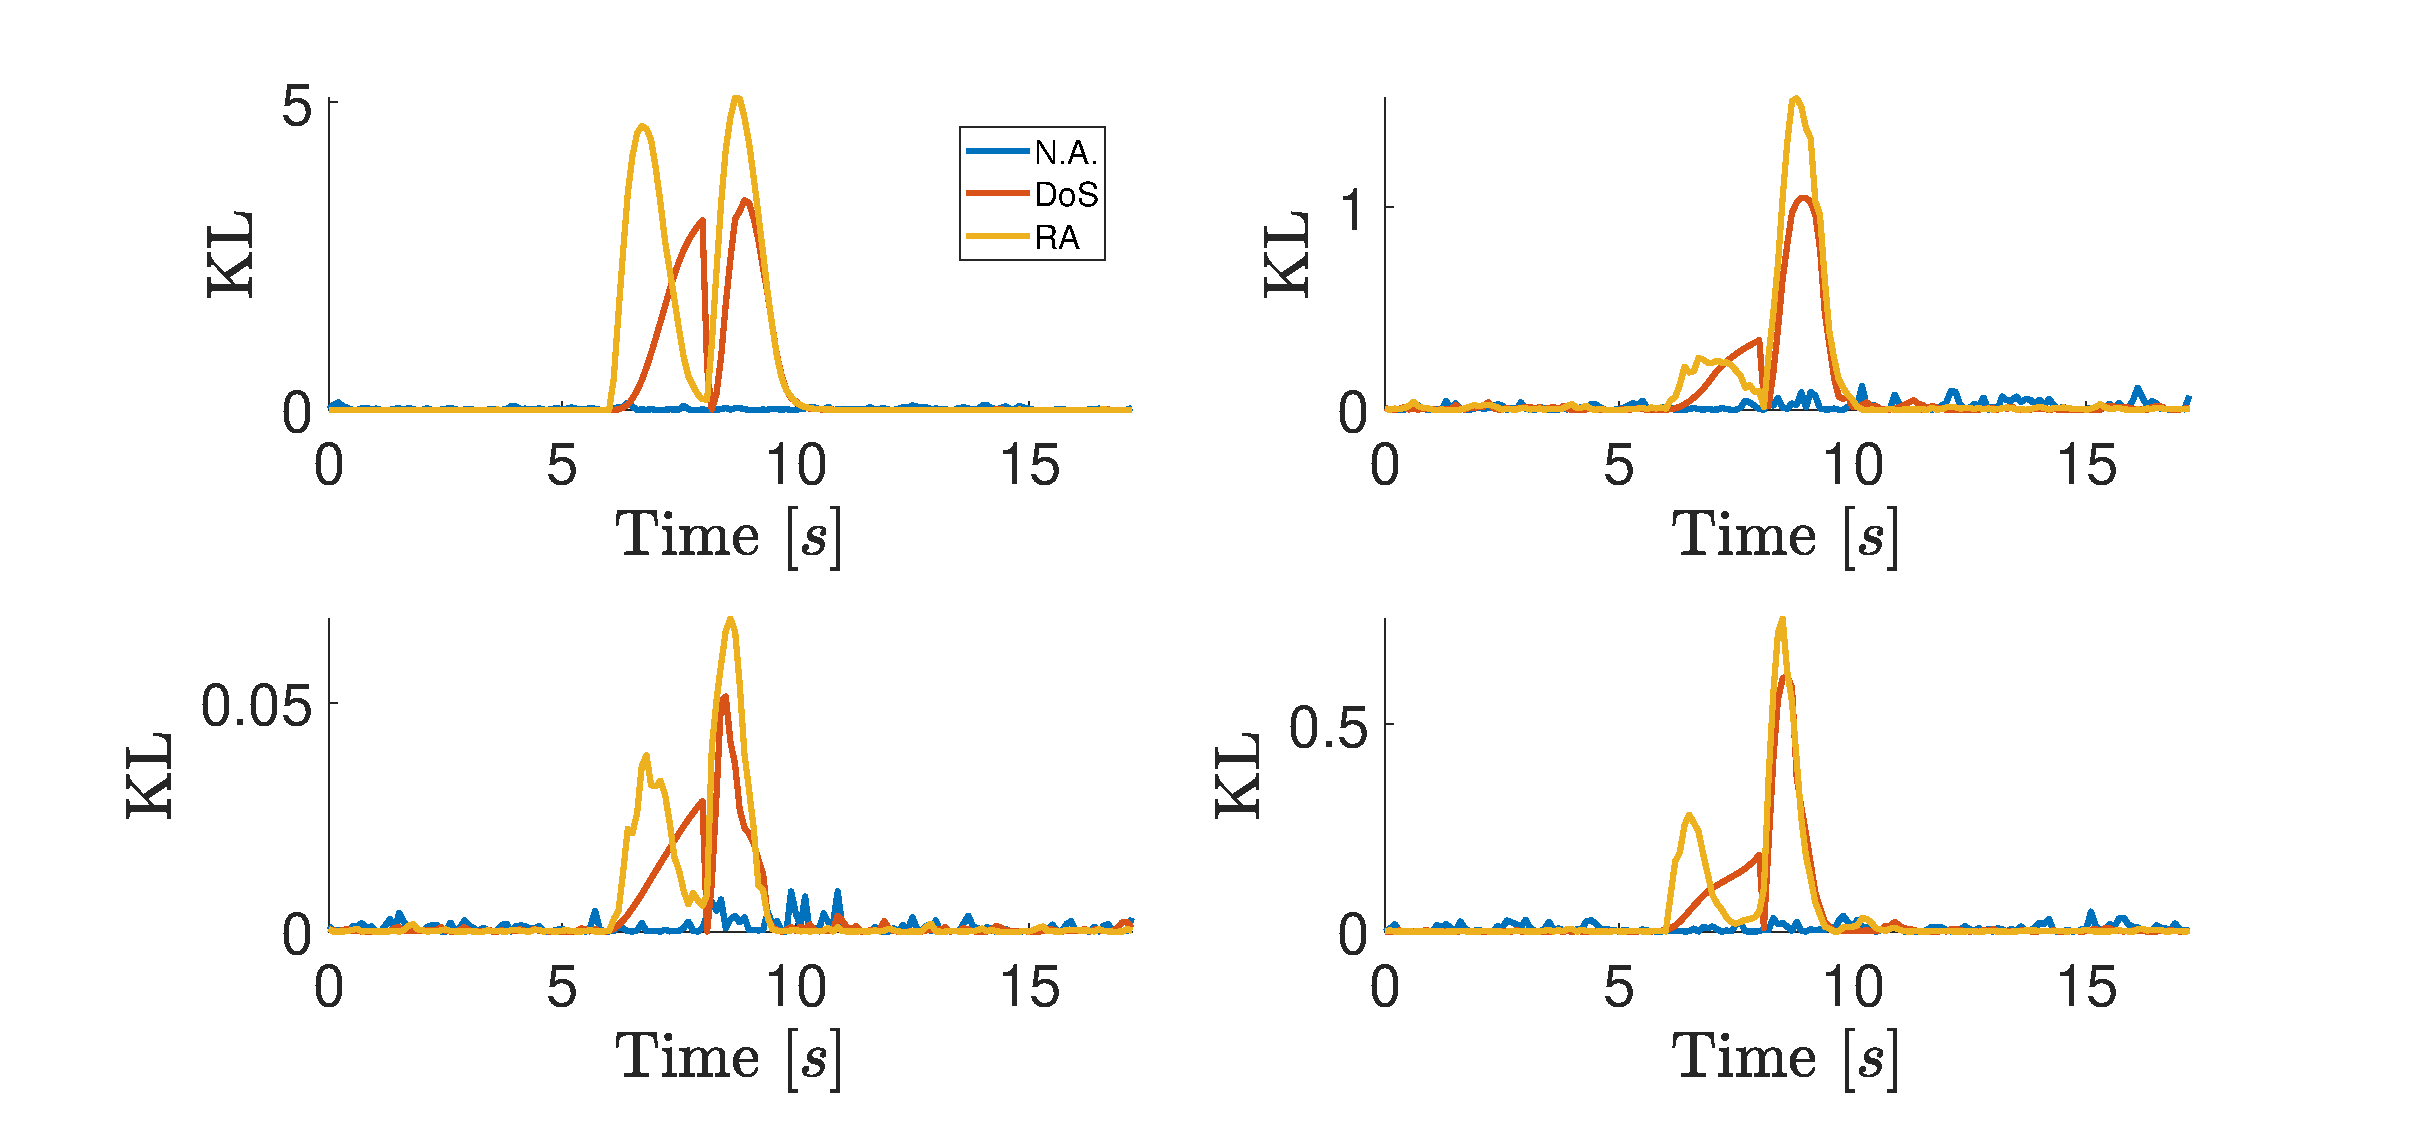
\includegraphics[scale=0.4]{figure/Part2/Chapter6/Figures/KL_All.eps}
	\caption{KL Divergences $D^{\mathrm{KL}}$. Top-left: $D^{\mathrm{KL}}\big(\bar{E}_x \| Q_x\big)$. Top-right: $D^{\mathrm{KL}}\big(\bar{E}_y \| Q_y\big)$. Bottom-left: $D^{\mathrm{KL}}\big(\bar{E}_\psi \| Q_\psi\big)$. Bottom-right: $D^{\mathrm{KL}}\big(\bar{E}_v \| Q_v\big)$. } 
	\label{fig:gamma_KL}
\end{figure}

\subsubsection{Classifier Training}
In order to build the attack dataset for the training of the detection model, for each class $N_{\rm sim}=10000$ simulations for the overtaking scenario have been carried out. Regarding the class~$0$, no attacks is injected all along the overtaking maneuver, whereas, regarding the other classes, the corresponding attack is injected. At the beginning of each attack,~$t_a$ and~$T_d$ are computed as realization of uniformly distributed random variables with supports~$\big[t^-_a, t^+_a\big]\subset\mathbb R^+$ and~$\big[T^-_d, T^+_d\big]\subset\mathbb R^+$, respectively. The features~\eqref{eq:J},~\eqref{eq:err} and \eqref{eq:kl_div} of the classes $1$-$6$ are collected during the attack phase \mbox{$t \in \big[t_a,t_a+ T_d\big]$}, while for the class $0$ the same features are collected during the whole time of the simulation.



The number of instances of each class during the training is reported in Table~\ref{table:classes}. In particular, the dataset is built such that in half of the instances there is an attack while no attacks are taking place in the rest.

The features $e_{\zeta}$, $J$ and $D^{\mathrm{KL}}$ during the training are reported respectively in Fig.~\ref{fig:gamma_error}--\ref{fig:gamma_KL}, where the Yellow lines refer to \gls{ra}, the Orange lines refer to DoS attacks and the Blue lines refer to no attacks (N.A.).

The confusion matrix of the \gls{csvm} Classifier is reported in Fig. \ref{fig:Confusion_matrix}, and Precision, Recall and F1 Score are reported in Table \ref{table:Best_classifier}.
%
\begin{figure}[h]
	\centering
	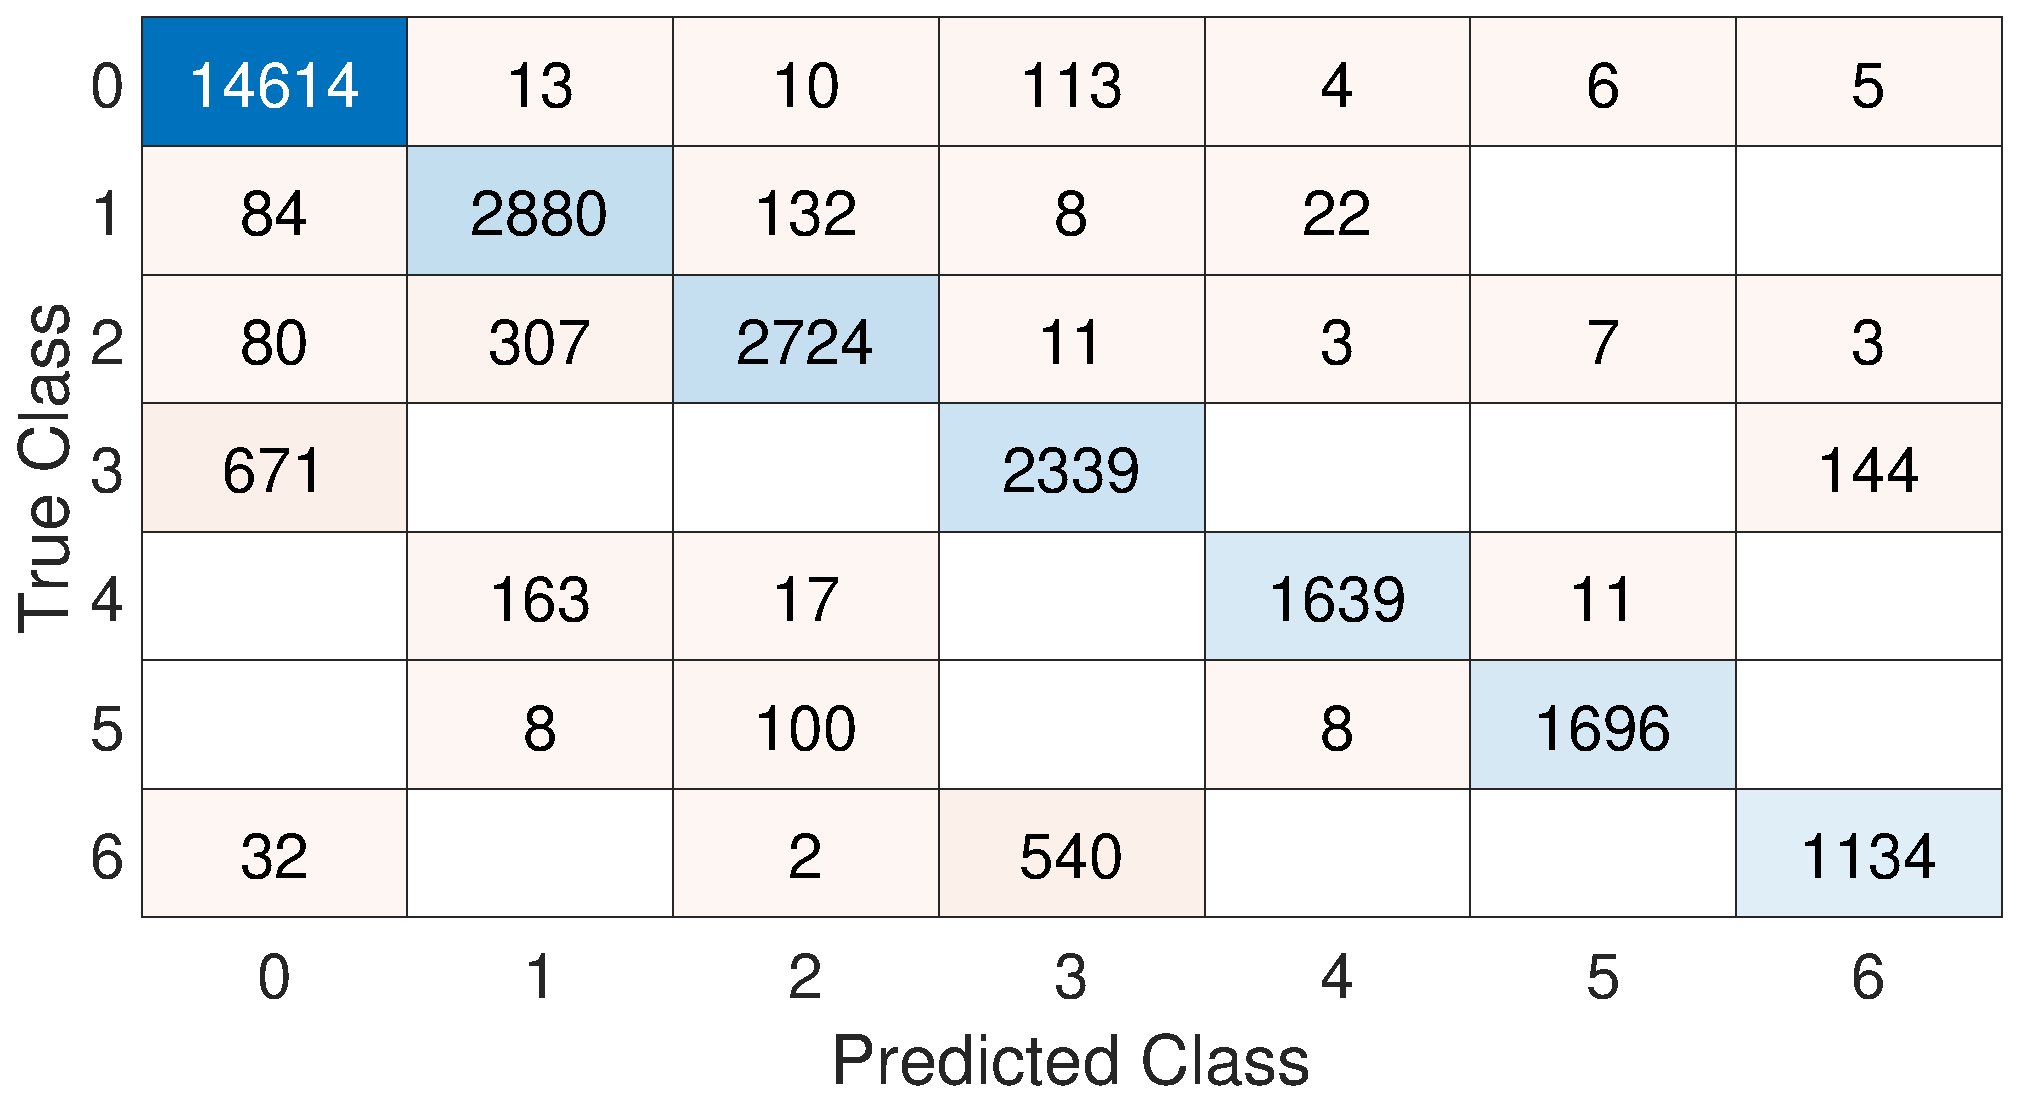
\includegraphics[scale=0.35]{figure/Part2/Chapter6/Figures/Confusion_matrix.eps}
	\caption{\gls{csvm} Confusion Matrix. }
	\label{fig:Confusion_matrix}
\end{figure}
%
%
%
%
In order to understand the effectiveness of the proposed approach we carried out a confrontation with the \gls{ra} Detector proposed in~\cite{detection_1} whose Precision, Recall and F1-Score result to be $81.6\%$, $35.1\%$ and $49.0\%$, respectively. While the proposed approach achieves Precision of $98.9\%$, Recall of $94.4\%$ and F1-Score of $96.6\%$. As it is possible to see, the obtained results show that the predictive features of the \gls{nmpc} could obtain satisfactory Classifier metrics. Regarding the metrics shown in Table~\ref{table:Best_classifier}, we remark that classes $2$ is less detectable compared to class $3$ and class $5$ is less detectable respect to class $6$, due to the different impact that the corresponding type of attack has on the performances of the control architecture.  
%
\begin{table}[h]
	\centering
	\begin{tabular}{ |c|c|c|c| } 
		\hline
		Classes  & Precision & Recall & F1 Score\\
		\hline
		\multirow{6}{2em}{\centering 0\\ 1\\ 2\\ 3\\ 4\\ 5\\ 6\\ } 
		& $94.4 \, \%$ & $99.0 \, \%$ & $ 0.96 $\\  
		& $85.4 \, \%$ & $92.1 \, \%$& $ 0.88 $ \\
		& $77.7 \, \%$ & $74.2 \, \%$& $ 0.75 $ \\
		& $91.3 \, \%$ & $86.9 \, \%$& $  0.89 $ \\ 
		& $97.8 \, \%$ & $89.6 \, \%$& $ 0.93 $ \\ 
		& $88.2 \, \%$ & $66.4 \, \%$& $ 0.75 $ \\ 
		& $98.6 \, \%$ & $93.6 \, \%$& $0.96 $ \\ 
		\hline
	\end{tabular}
	\vspace{0.25 cm}
	\caption{Cubic SVM Classifier.}
	\label{table:Best_classifier}
\end{table}
%%% END SECTION ============================================================

%%% START SECTION ==========================================================

\section{Simulations and results}
\label{sec:fourth}
%
In this section we present the simulation outcomes of the proposed scheme in comparison with those of a \gls{av} architecture where no mitigation is considered. The software is implemented in MATLAB\textsuperscript{\textregistered} and CasADi~\cite{Casadi}, and the simulation parameters are reported in Table~\ref{tab:parameters}.
%
\begin{table}[ht]
	\centering
	\begin{tabular}[ht]{|l|l|c|}
		\hline
		\textbf{Parameters} & \textbf{Value}\\
		\hline
		$l_f$& \SI{1.738}{\metre}\\
		$l_r$& \SI{1.105}{\metre}\\
		$T_s$& \SI{0.1}{\second}\\
		$S$&  $\mathrm{diag}\big(100,1000\big)$ \\
		$R$& $\mathrm{diag}\big(0.1,0.1\big)$\\
		$L$& $\mathrm{diag}\big(10,10,400,200\big)$ \\
		$\dot{u}_{{\rm max}}$& $\begin{bmatrix}\SI{0.6}{{\metre}/{\second^3}} & \SI{0.2}{{\radian}/{\second}}\end{bmatrix}^\top$ \\
		$\dot{u}_{{ \rm min}}$& $\begin{bmatrix}\SI{-0.6}{{\metre}/{\second^3}} & \SI{-0.2}{{\radian}/{\second}}\end{bmatrix}^\top$ \\
		${u}_{{ \rm max}}$&$\begin{bmatrix}\SI{2.5}{{\metre}/{\second^2}} & \SI{0.7}{\radian}\end{bmatrix}^\top$\\
		${u}_{{ \rm min}}$& $\begin{bmatrix}\SI{-2.5}{{\metre}/{\second^2}} & \SI{-0.7}{\radian}\end{bmatrix}^\top$ \\
		$H_p$& 30 \\
		$N_M$& 15 \\
		\hline
	\end{tabular}
	\caption{Parameter values.}
	\label{tab:parameters}
\end{table}%
%
%	 
In \mbox{Fig.~\ref{fig:no_attack}-\ref{fig:MPC_dos}}, the simulations regarding the overtaking maneuver are reported in case no mitigation countermeasure is implemented. Cyan lines refer to the trajectory references, orange lines refer to the state measurements and Yellow lines refer to the state estimates. Only attacks on the entire attack space have been considered with $t_a= \SI{9.5}{\second}$ and $T_d=\SI{2}{\second}$ for \glspl{ra} and $t_a= \SI{7.5}{\second}$ and $T_d=\SI{2}{\second}$ for \gls{dos} attacks. For different values of $t_a \in \big[t^-_a, t^+_a\big]$ the Detector behaviour is the same. 

In Figs.~\ref{fig:MPC_RA},~\ref{fig:MPC_dos} it is possible to note that  the error between the measured/actual $x$ and $y$ and the reference in \glspl{ra} is greater than in \gls{dos} attacks, thus implying a higher control degradation. This happens because in \gls{dos} attacks only the state in the last sampling interval is available while in \glspl{ra} a replayed state sequence is available that is related to a time window spanning several samples back in time. Reintroduce these past state estimate sequence to the \gls{nmpc} produces a considerable error in the calculation of the control inputs; 
in particular, the greater the replay time, the more evident the degradation of performance is.

The effectiveness of the \gls{imps} architecture is shown in \mbox{Fig.~\ref{fig:Simulation_Mitigator}} where the heading angle, the velocity and the position are reported when an \gls{ra} with  $t_a= \SI{10}{\second}$ and $T_d=\SI{2}{\second}$. As it is possible to notice, the implemented \gls{imps} is able to detect in time the cyber-attack and the mitigation action allows the \gls{av} to conduct an overtaking maneuver safely. Indeed, the safety of the maneuver is obtained by minimizing the position error with respect to the trajectory planned by the planner. Furthermore, the time to detect the attacks is of two time steps.

The effectiveness of proposed architecture is also highlighted in Fig.~\ref{fig:Safe_set} which reports the trajectories in the $e_x-e_y$ plane for an AV during overtaking when both the proposed scheme is implemented and the proposed scheme is not implemented. An ellipsoidal safe region for the overtaking maneuver is also plotted (solid red line) and the trajectory position errors are reported for the aforementioned simulations. The safe region is computed as the maximum deviation with respect to the trajectory reference which allows the \gls{av} to perform the overtaking maneuver without damaging or hitting possible obstacles.

Cyan, Magenta, Green and Blue represent the simulations regarding No Attack, \gls{ra} with \gls{imps}, \gls{dos} attack and \gls{ra} without \gls{imps}, respectively. The novel \gls{imps} implemented allows to reduce the effect of cyber-attacks generated by a hacker. In cases of no detection and mitigation of \gls{ra} and \gls{dos} attack, the errors of the trajectory result out of the safety region, which could cause damages and possible injuries to the driver.
%
\begin{figure}
	\centering
	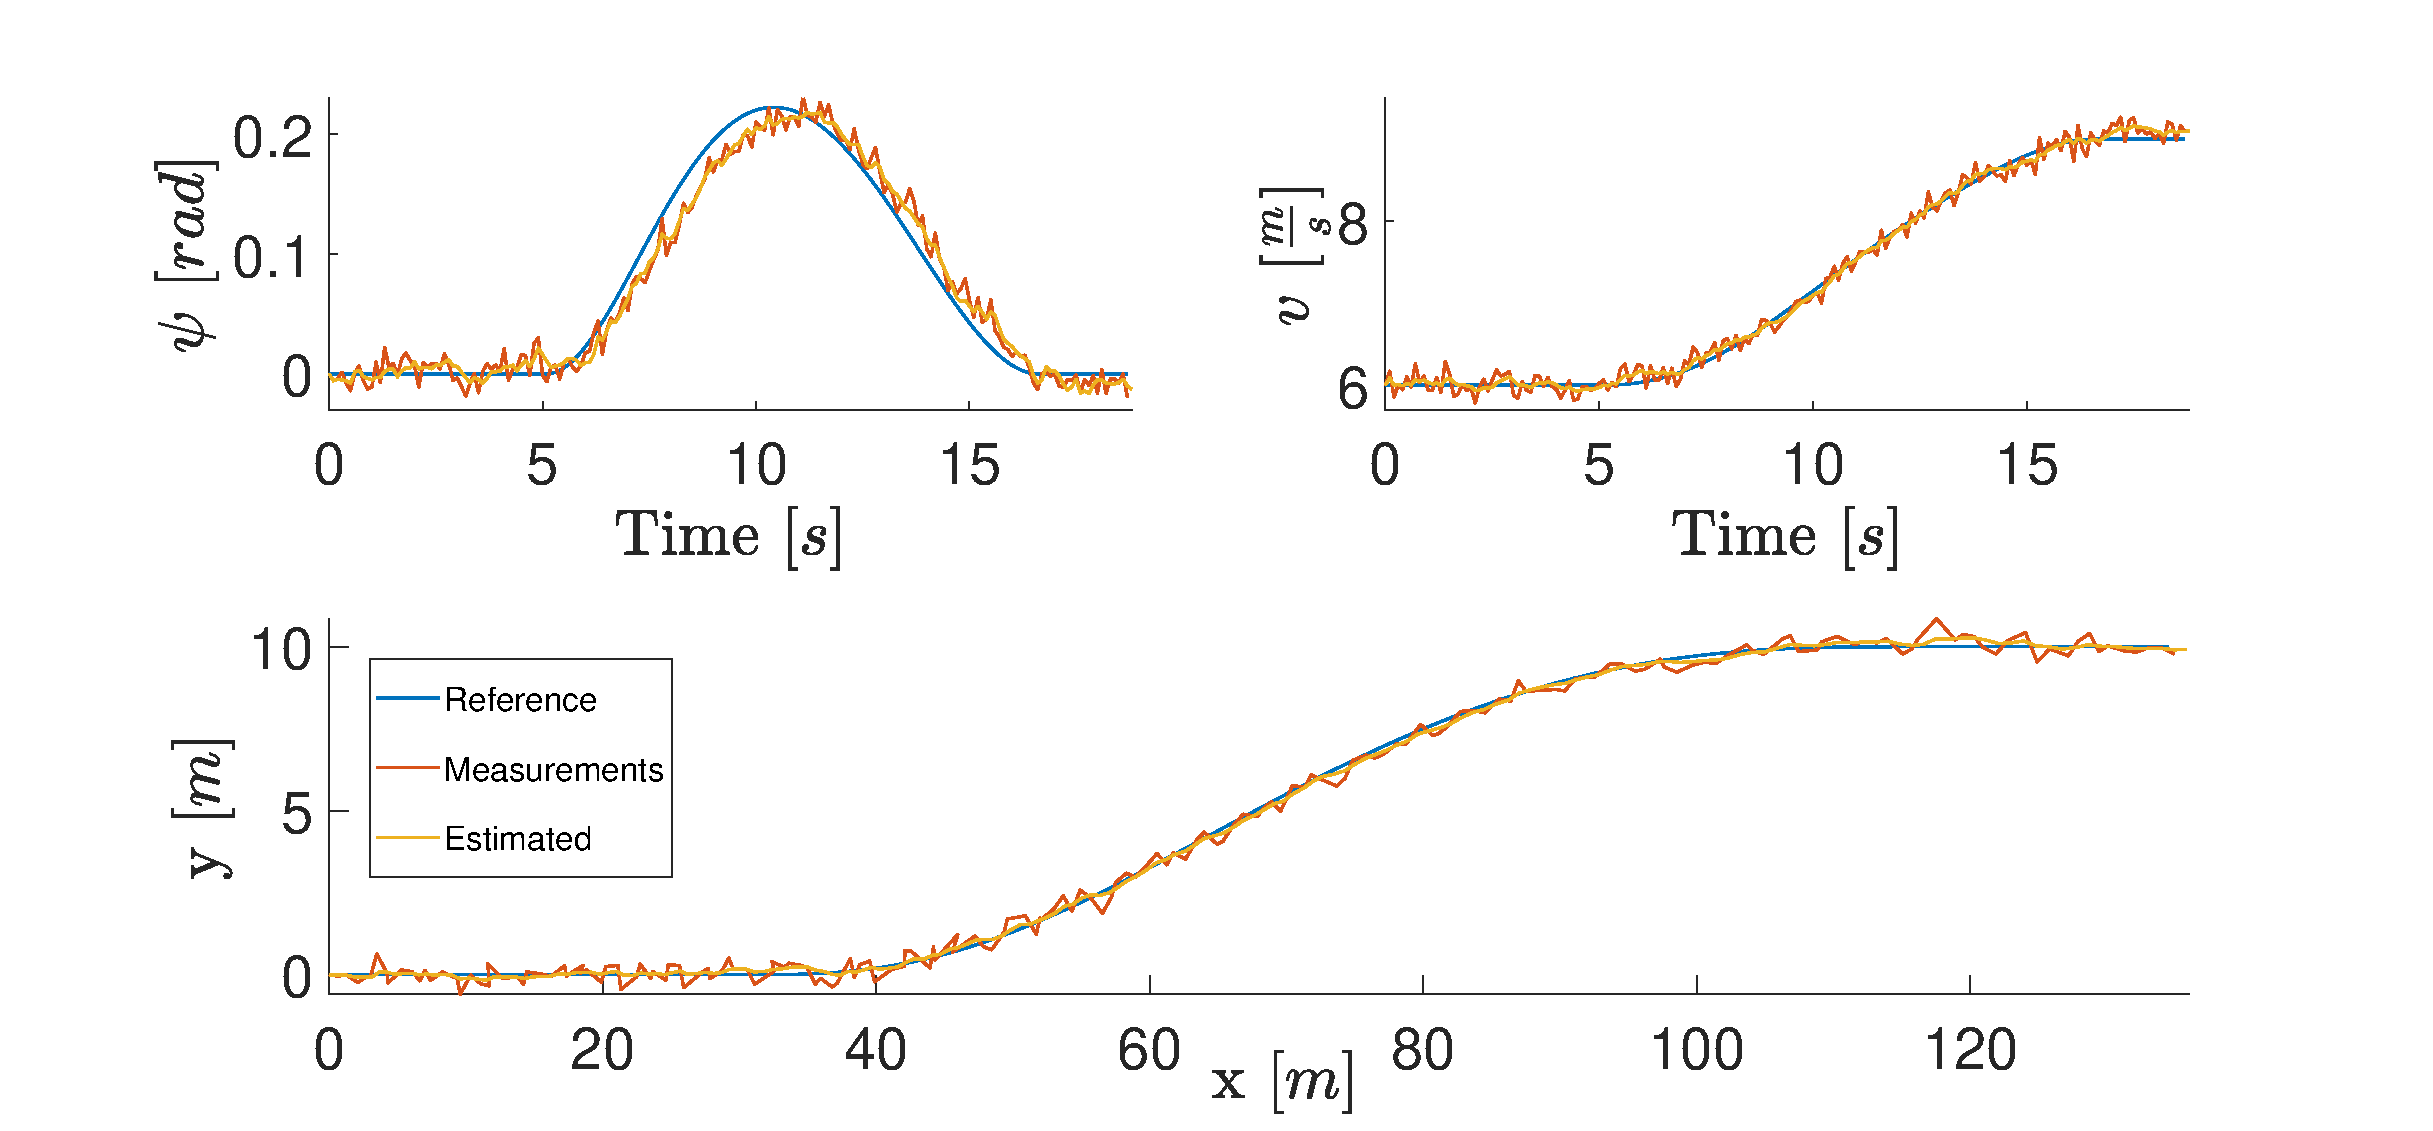
\includegraphics[scale=0.4]{figure/Part2/Chapter6/Figures/MPC.eps}
	\caption{No attacks.}
	\label{fig:no_attack}
\end{figure}
%
\begin{figure}
	\centering
	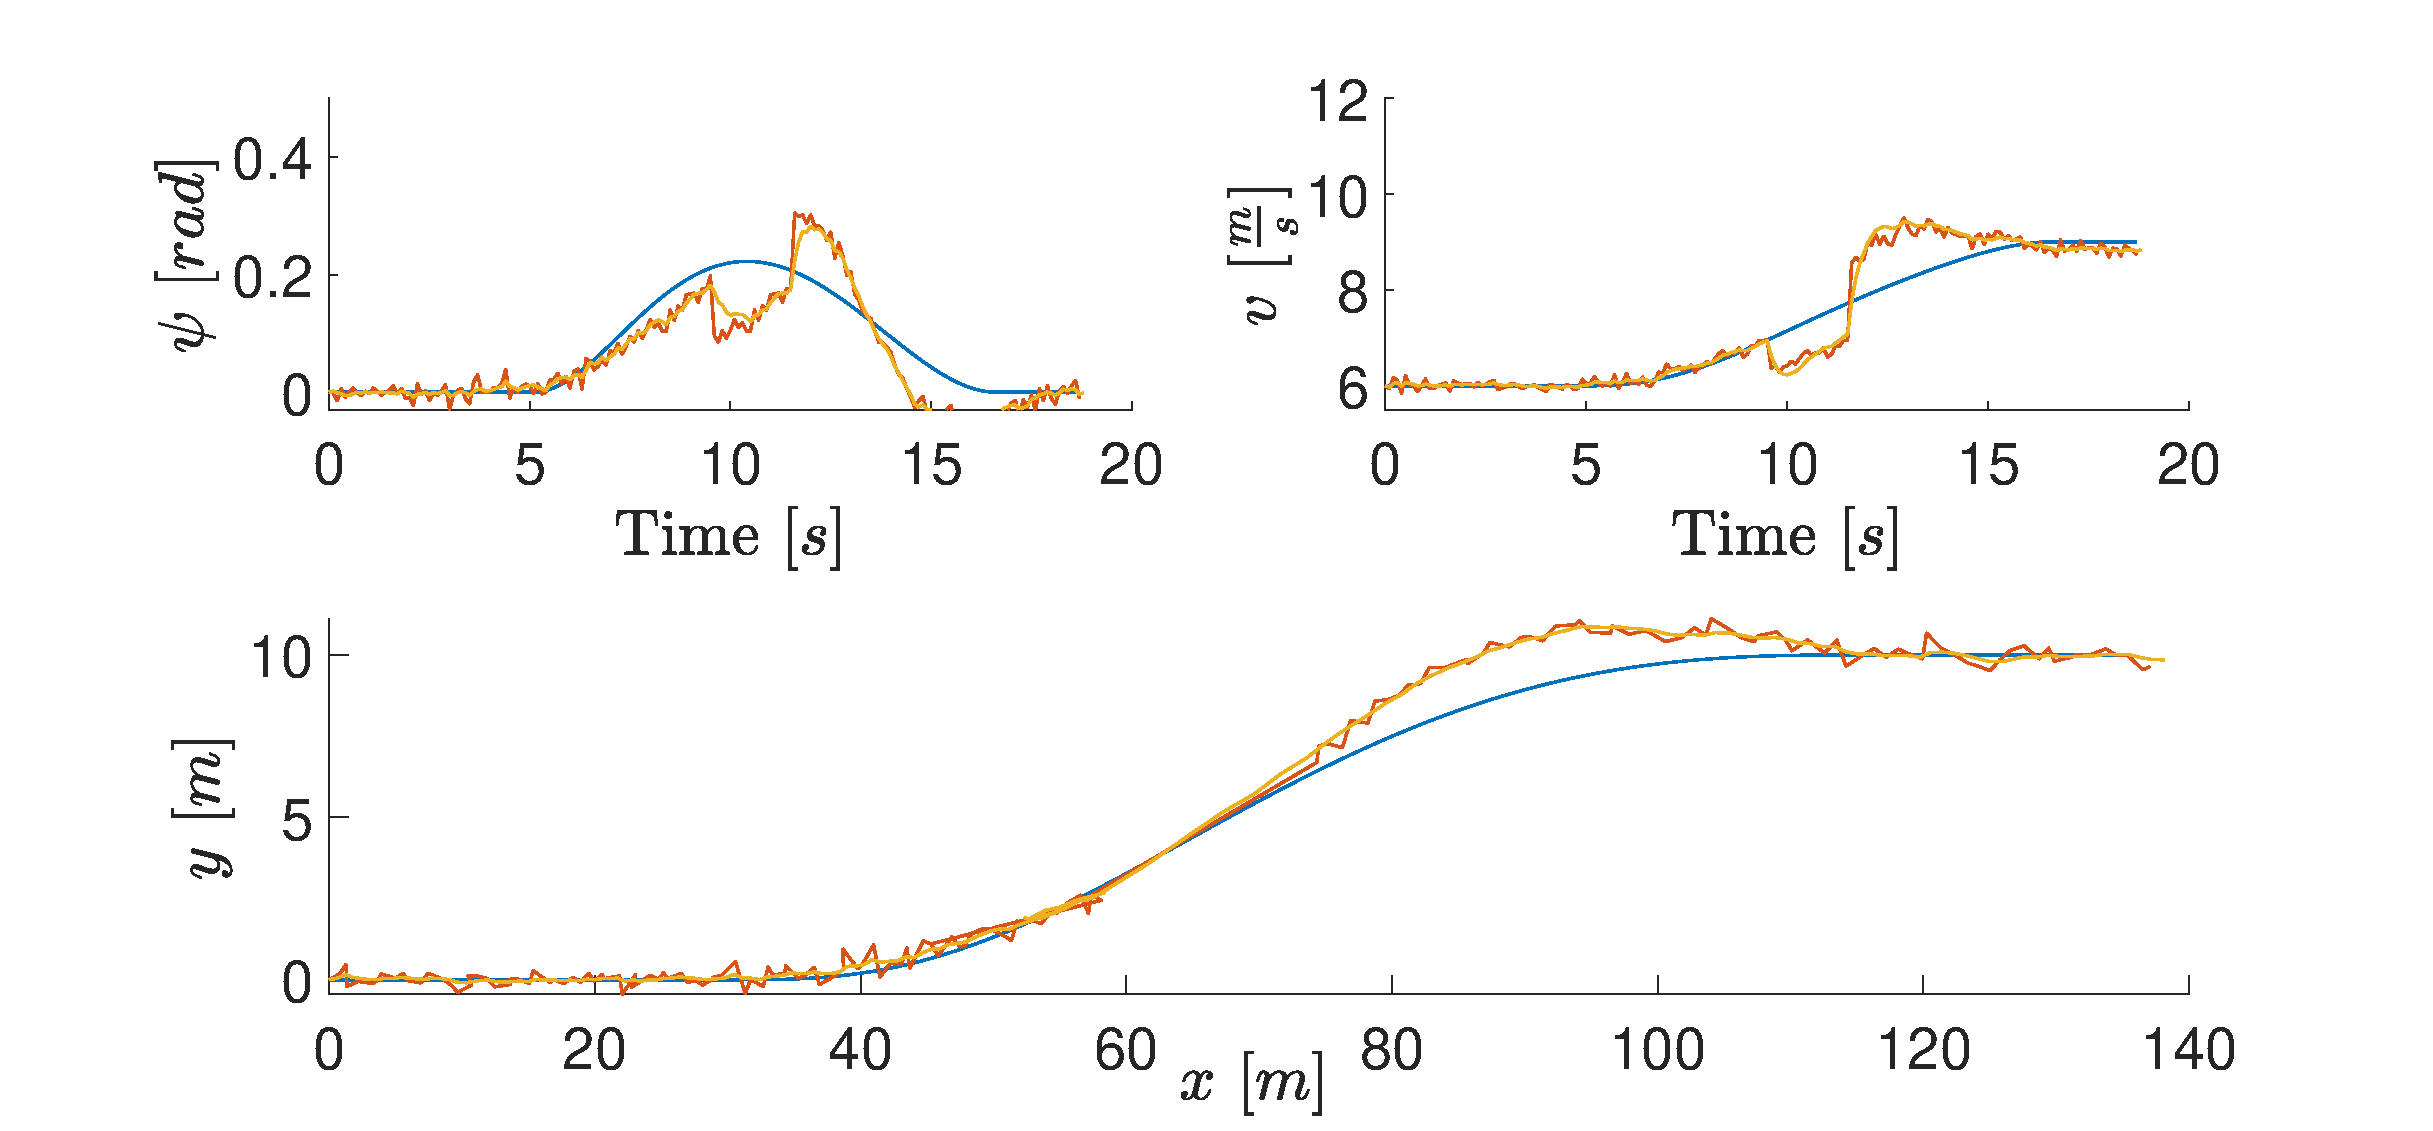
\includegraphics[scale=0.4]{figure/Part2/Chapter6/Figures/MPC_Replay.eps}
	\caption{\gls{ra}.}
	\label{fig:MPC_RA}
\end{figure}
%
\begin{figure}
	\centering
	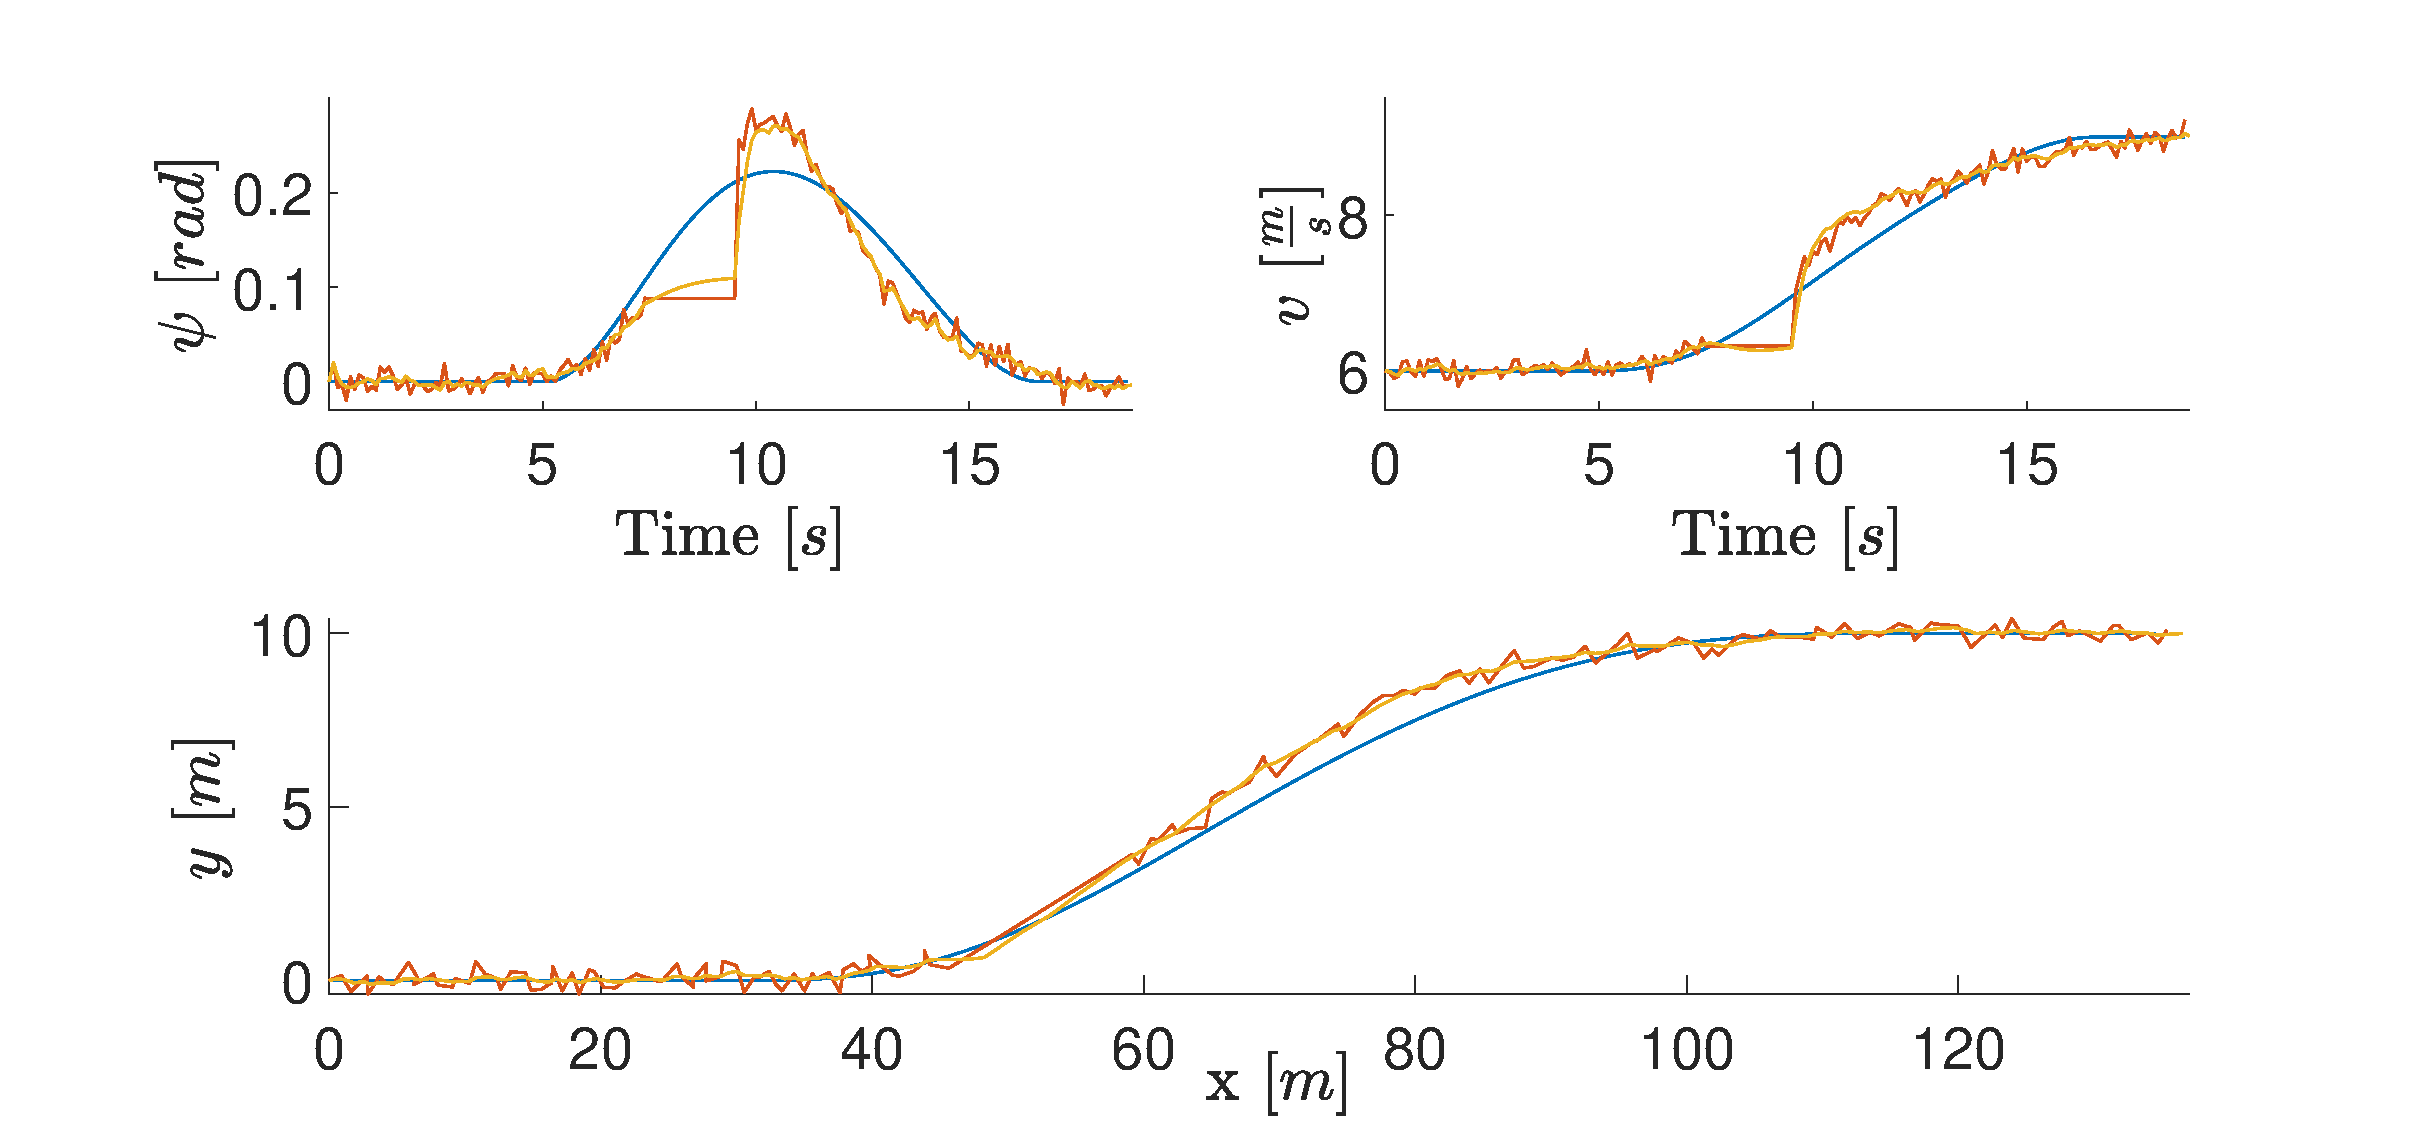
\includegraphics[scale=0.4]{figure/Part2/Chapter6/Figures/MPC_DoS.eps}
	\caption{\gls{dos} attack.}
	\label{fig:MPC_dos}
\end{figure}

%


\begin{figure}
	\centering
	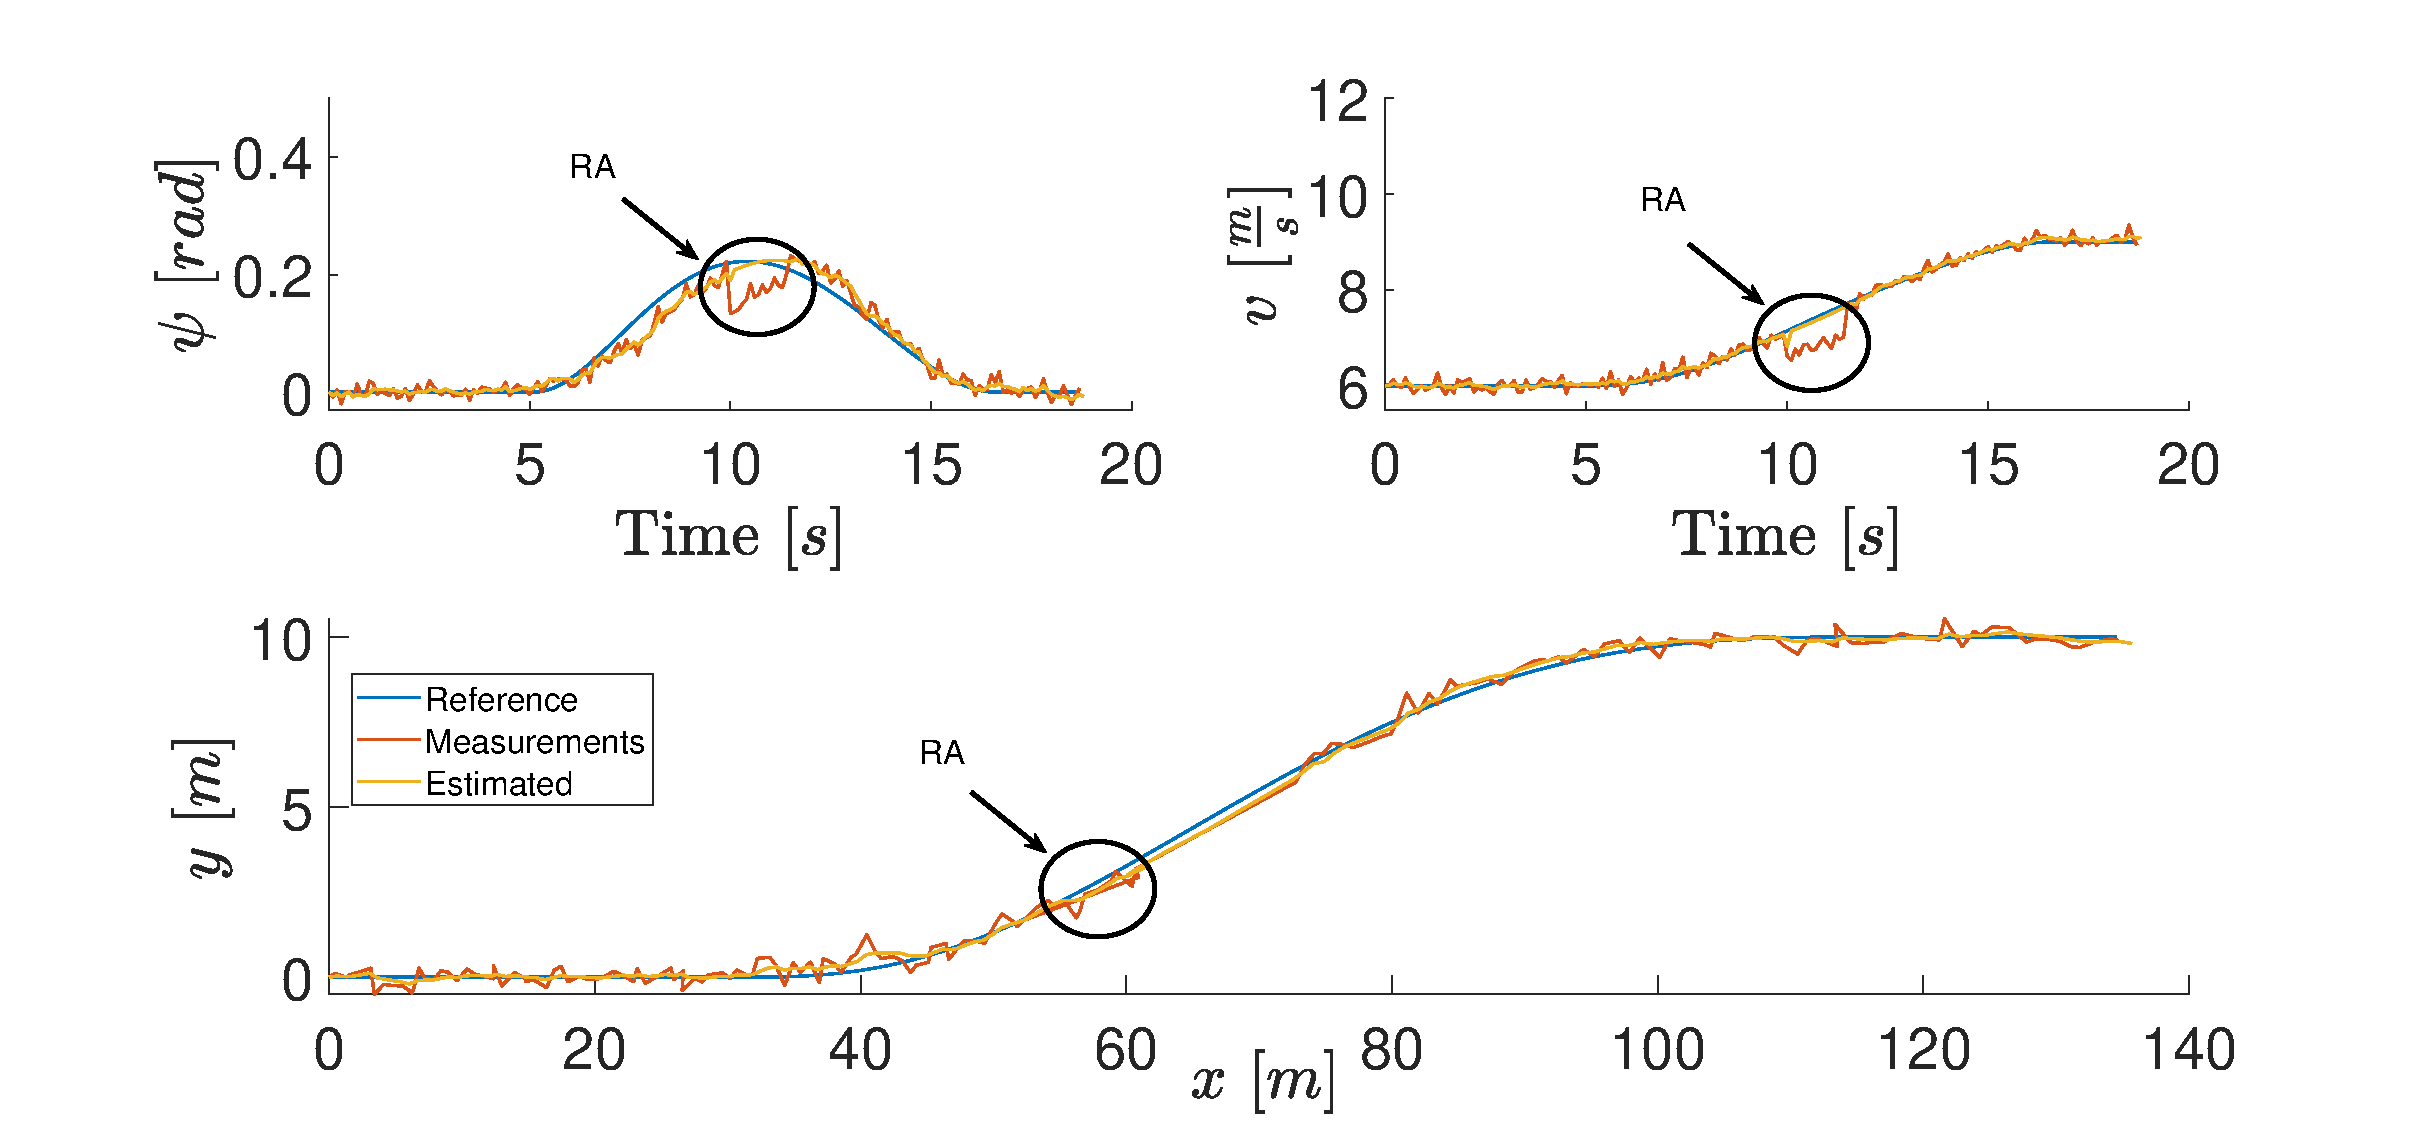
\includegraphics[scale=0.4]{figure/Part2/Chapter6/Figures/Mitigation_fin.eps}
	\caption{\gls{ra} mitigation using \gls{imps}. Start time attack and duration are  $t_a= \SI{10}{\second}$ and $T_d=\SI{2}{\second}$, respectively. Top-left: Heading angle. Top-right: Velocity. Bottom: Position.   }
	\label{fig:Simulation_Mitigator}
\end{figure}
%
\begin{figure}
	\centering
	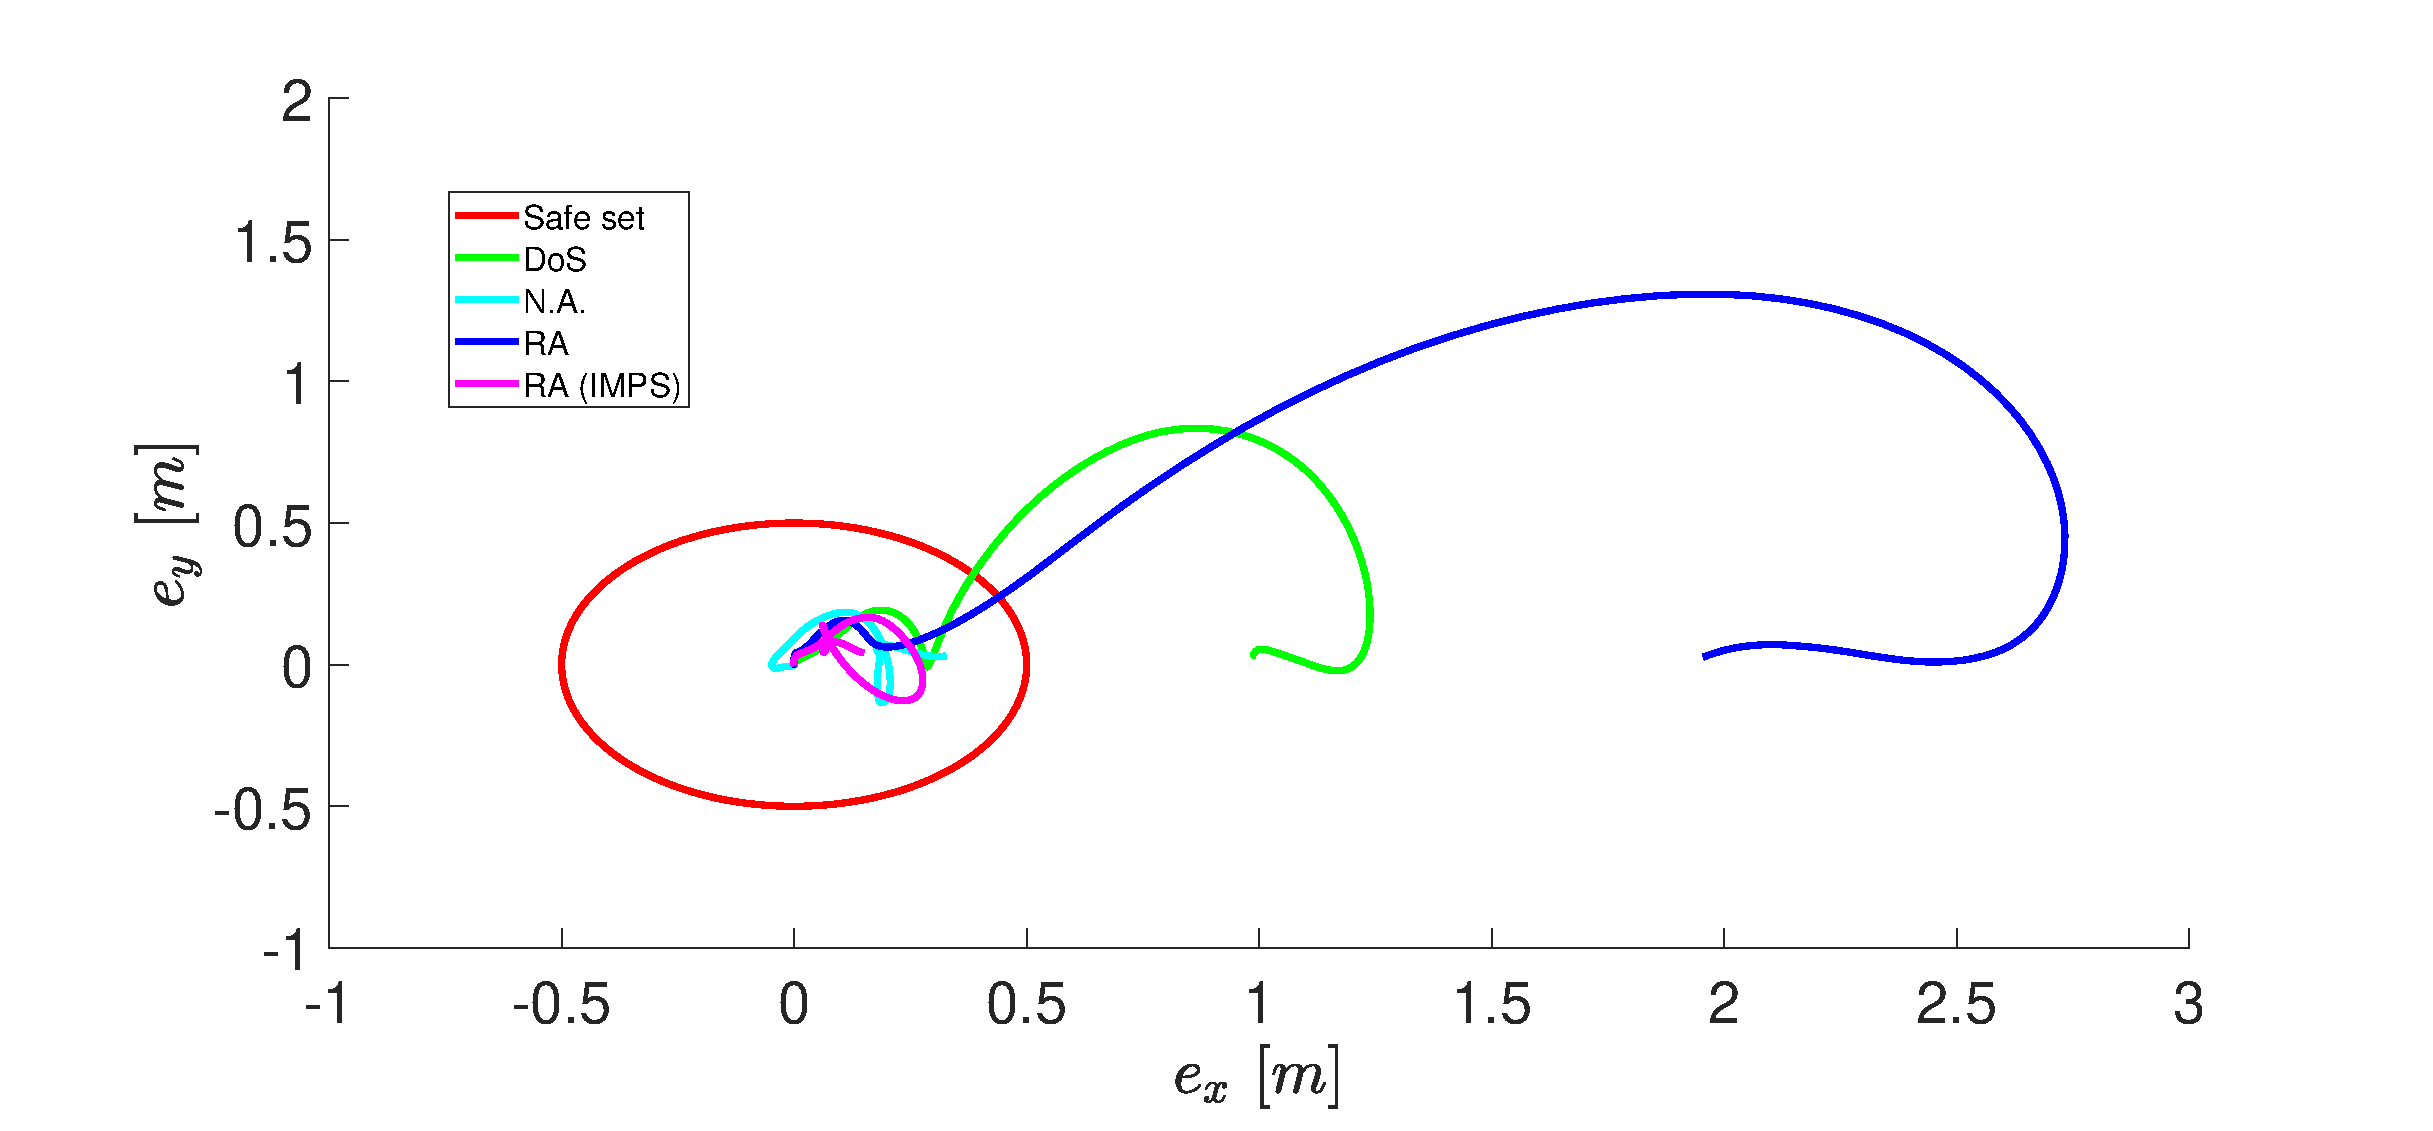
\includegraphics[scale=0.4]{figure/Part2/Chapter6/Figures/Safe_set.eps}
	\caption{Safe region and error trajectories. }
	\label{fig:Safe_set}
\end{figure}
%




\clearpage
\section{Chapter Summary}


The conclusion of this chapter highlights the Informative Model Predictive Scheme algorithm's successful application in enhancing cybersecurity for autonomous vehicle systems, particularly during overtaking maneuvers vulnerable to cyber-attacks such as Replay Attacks and Denial of Service. Numerical results from simulations validate the efficacy of the I-MPS, demonstrating its potential in accurately detecting and mitigating cyber threats in real-time. These findings suggest a significant step forward in vehicular cybersecurity, illustrating the innovative synergy between machine learning algorithms and control systems in combatting cyberattacks. The results also indicate areas for further accuracy enhancement, reinforcing the I-MPS as a pioneering approach in the ongoing evolution of cybersecurity measures for autonomous vehicles.